\chapter{实验结果与分析}

\section{ELISA检测体系的建立与评价}

\subsection{ELISA检测体系的设计思路}

本研究的核心目标是建立能够定量反映HBV核心蛋白（HBc）与HBsAg preS区域相互作用的体外检测体系，并为后续比较preS突变体及小分子抑制剂的影响奠定基础。根据前期结构研究，preS 87--114片段是与HBV核衣壳结合的关键区域。因此，本研究首先围绕HBc与preS片段的互作检测进行了方法学探索。

考虑到HBc--preS相互作用可能较弱，且容易受到固定化方式、蛋白取向和洗涤步骤影响，本研究前期比较了多种ELISA模式。三类ELISA体系分别从不同角度优化互作检测：其一，直接包被HBc颗粒，再检测结合到HBc上的preS；其二，通过StrepXT定向捕获带Strep标签的preS，再加入HBc并检测结合的核心蛋白；其三，通过抗HBc Fab捕获HBc颗粒，再检测preS结合。通过比较这些模式的信号窗口、背景水平和重复性，可以判断传统固相ELISA是否适合作为后续突变体和小分子筛选平台。

\subsection{HBVCp149的表达与纯化}

为建立HBc--preS互作检测体系，首先需要获得可用于包被或捕获实验的HBV核心蛋白样品。本研究使用截短形式的HBVCp149蛋白作为实验样品。经分步盐析和Q柱阴离子层析后，HBVCp149在主要洗脱组分中呈现清晰的目标条带，说明目标蛋白得到有效富集。层析曲线中主要峰较为明显，同时伴随两个较小的肩峰，提示样品中可能存在少量不同装配状态的核心蛋白或杂质组分；但用于后续实验的合并组分在SDS-PAGE中整体较为干净，能够满足ELISA包被和定量滴定的需要。

这一结果说明，HBVCp149的表达和纯化流程可以稳定获得后续体外互作分析所需的核心蛋白材料。由于HBc的颗粒状态和表面构象对preS结合具有重要影响，后续ELISA重点比较了不同固定化方式能否在尽量保留互作界面的同时产生足够稳定的特异信号。

\begin{figure}[htbp]
  \centering
  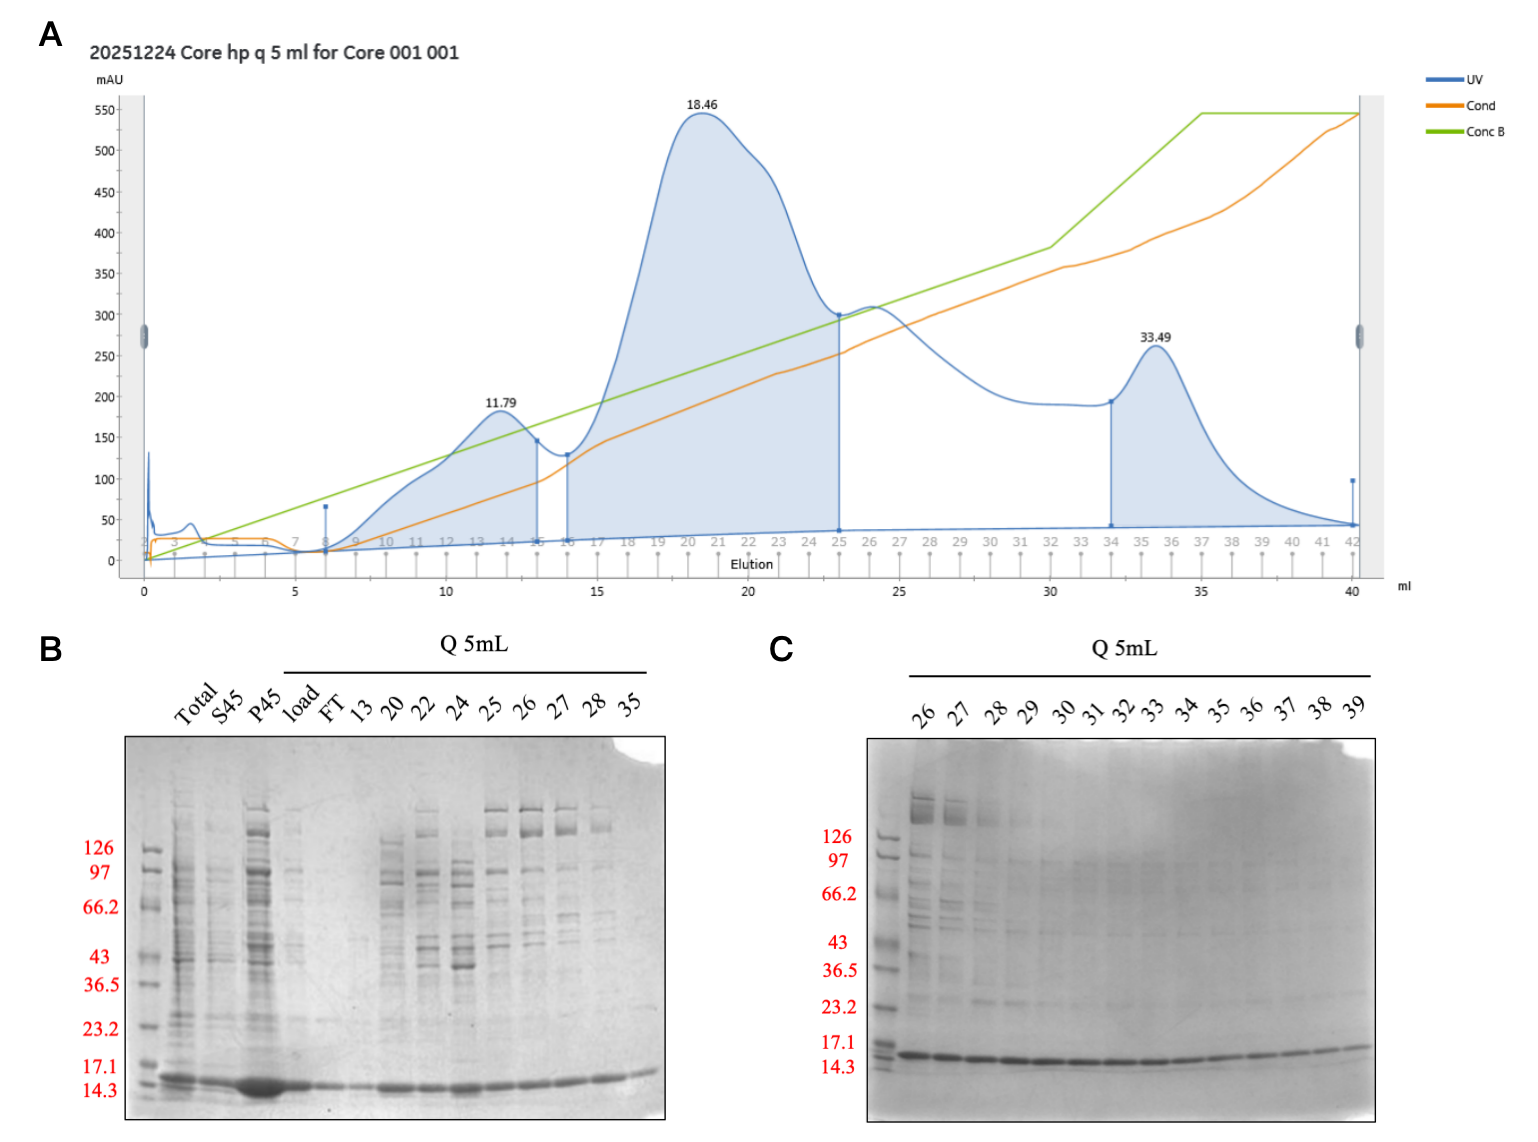
\includegraphics[width=1.0\textwidth]{docs/figures/result/result_01_hbvcp149.png}
  \caption{HBVCp149的表达与纯化结果。A，HBVCp149的Q HP阴离子层析柱层析曲线。B、C，不同组分的SDS-PAGE分析，目标核心蛋白在主要洗脱组分中得到富集，可用于后续ELISA检测。}
  \label{fig:hbvcp149-purification}
\end{figure}

\subsection{ELISA模式一：HBc直接包被}

在第一种ELISA模式中，HBVCp149被直接包被于酶标板表面，随后加入带标签的preS蛋白，并通过抗标签抗体检测结合到板上的preS信号。该设计的优点是检测路径较短，理论上能够直接反映preS与固定化HBc之间的结合；但其潜在问题是核心蛋白直接吸附到塑料表面后，颗粒构象或preS结合面可能受到影响，同时preS和检测抗体也可能产生非特异吸附。

首先对HBVCp149包被量进行滴定，结果显示扣除背景后的特异信号呈现可饱和趋势，且能够较好地用Langmuir单点吸附模型拟合，提示HBc直接包被在技术上具有一定可重复性。根据包被曲线，后续实验选择20 nM HBVCp149作为工作浓度。

然而，在该条件下进一步滴定preS时，实验组的特异信号仅轻微升高，整体仍接近基线；同时，在未包被HBc的对照孔中仍可保留较高的总信号。20 nM HBc组与0 nM HBc组之间分离度有限，说明该体系的读数主要受到preS或抗体在板面上的非特异吸附影响，而不是由稳定的HBc--preS特异结合主导。

\begin{figure}[htbp]
  \centering
  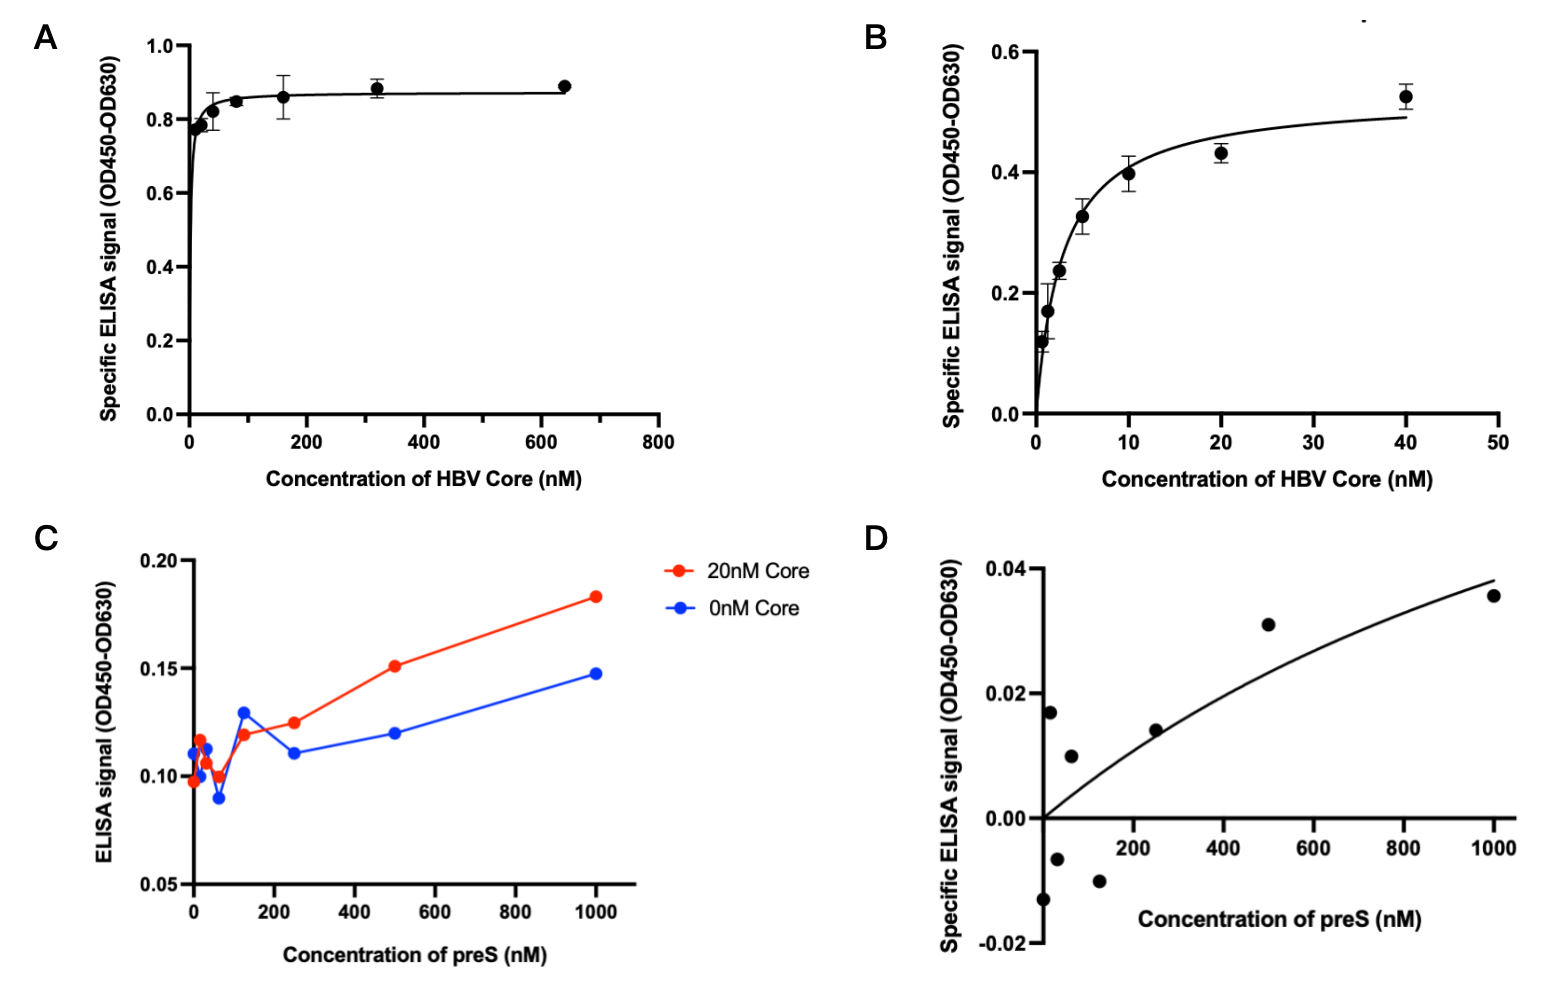
\includegraphics[width=1.0\textwidth]{docs/figures/result/result_02_elisa_a.png}
  \caption{HBc直接包被的ELISA的检测结果。A、B，HBVCp149包被滴定可获得可饱和信号。C、D，在固定HBc后检测preS结合时，实验组与无HBc对照组分离有限，提示该构型受到非特异吸附背景影响。}
  \label{fig:elisa-format-a}
\end{figure}

因此，HBc直接包被ELISA虽然步骤简单，但不能提供足够清晰的HBc依赖性信号窗口。该结果提示，后续体系需要减少preS直接接触塑料表面的机会，并尽量通过定向捕获方式改善preS呈递。

\subsection{ELISA模式二：StrepXT捕获preS}

为降低preS直接吸附造成的背景，本研究进一步构建了StrepXT捕获preS的ELISA模式。在该体系中，酶标板首先包被StrepXT，随后通过Strep标签定向捕获preS，再加入HBVCp149，最后通过抗HBc抗体检测结合到preS上的核心蛋白。与直接包被HBc的体系相比，该构型的主要优势在于preS可以通过标签被定向固定，从而提高其可及性并降低随机吸附带来的背景。

首先对StrepXT进行了表达纯化和功能评估。经包涵体回收、变性复性和Q柱阴离子层析纯化后，StrepXT在洗脱组分中出现相对富集的目标条带，说明目标蛋白已从主要杂质中分离出来。进一步测定其有效结合位点，平均有效值约为0.852，提示StrepXT复性后保留了较好的Strep标签捕获能力，可用于后续preS定向固定实验。

\begin{figure}[htbp]
  \centering
  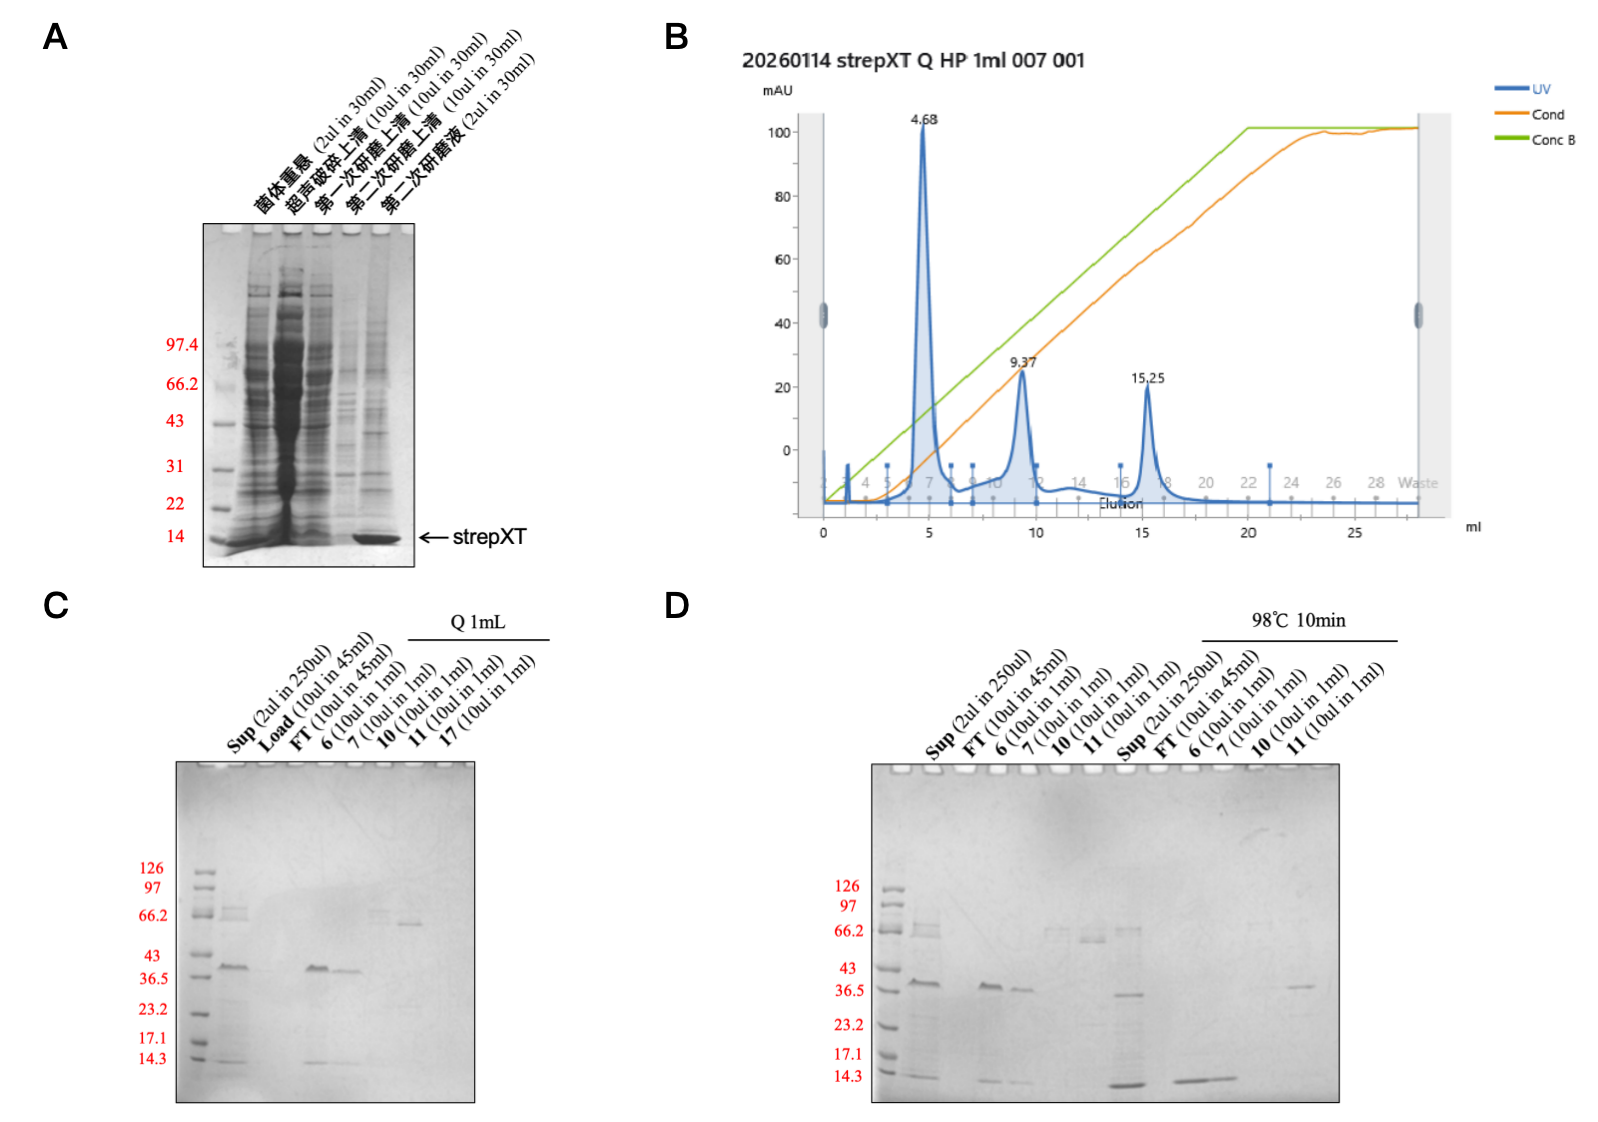
\includegraphics[width=1.0\textwidth]{docs/figures/result/result_03_strepXT.png}
  \caption{StrepXT的表达纯化与功能评估。A，透析前各组分的SDS-PAGE分析。B，StrepXT的Q HP阴离子层析柱层析曲线。C、D，阴离子层析后各组分的SDS-PAGE分析，结果显示StrepXT在洗脱组分中得到富集；结合位点定量结果表明复性后的StrepXT具有较好的Strep标签捕获能力。}
  \label{fig:strepx-purification}
\end{figure}

在StrepXT捕获体系中，50 nM StrepXT能够较稳定地包被于板面并捕获带Strep标签的preS。preS滴定曲线呈现典型的可饱和趋势，且能够较好地用Langmuir单点吸附模型拟合，说明该体系能够有效控制preS本身的呈递过程。基于该结果，后续HBVCp149结合实验中选择100 nM preS作为工作浓度。与HBc直接包被体系相比，StrepXT捕获明显改善了preS固定化方式，说明模式一中的部分背景确实来源于preS在板面上的非特异吸附。

然而，在HBc结合实验中，核心蛋白检测信号仍然非常分散，信噪比过低，特异信号窗口几乎不可见。推测这可能是因为用于检测的抗HBc抗体的特异性过低，因此进一步制备了特异性较高的抗HBc IgG重复实验，希望可以提高信号的特异性。

\begin{figure}[htbp]
  \centering
  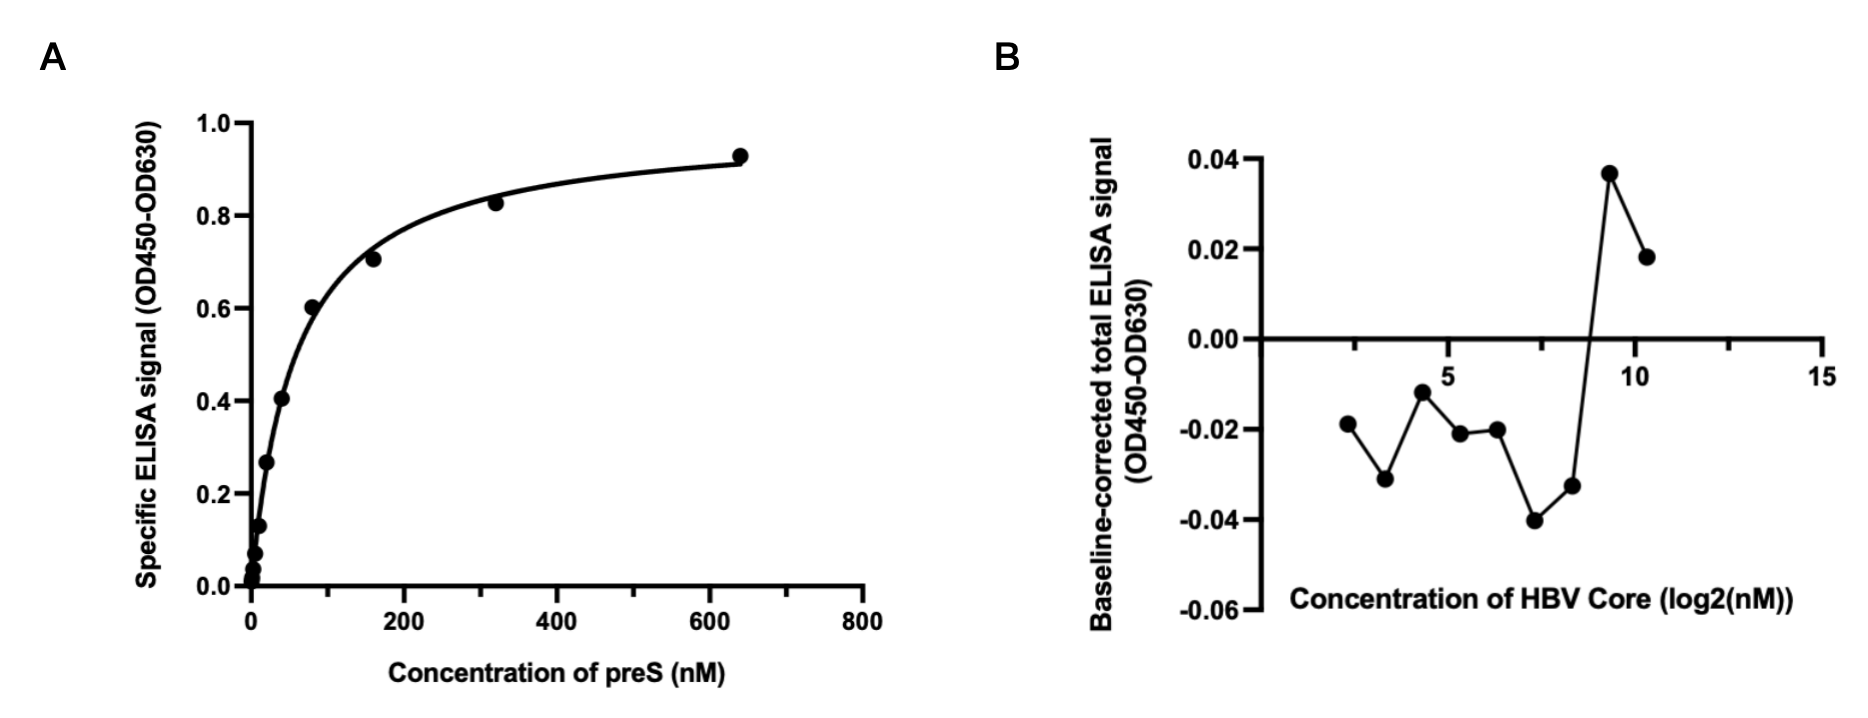
\includegraphics[width=1.0\textwidth]{docs/figures/result/result_04_elisa_b_1.png}
  \caption{StrepXT捕获preS的ELISA模式的初步检测结果。A，preS捕获滴定呈现可饱和曲线，说明preS呈递得到改善。B，HBV核心蛋白结合检测的特异信号仍较弱且波动较大。}
  \label{fig:elisa-format-b-initial}
\end{figure}

SDS-PAGE结果显示，IgG D4在还原条件下具有清晰的重链和轻链条带，在非还原条件下可见完整IgG条带，说明该抗体成功表达和纯化。后续实验使用IgG D4替代原检测抗体。

\begin{figure}[htbp]
  \centering
  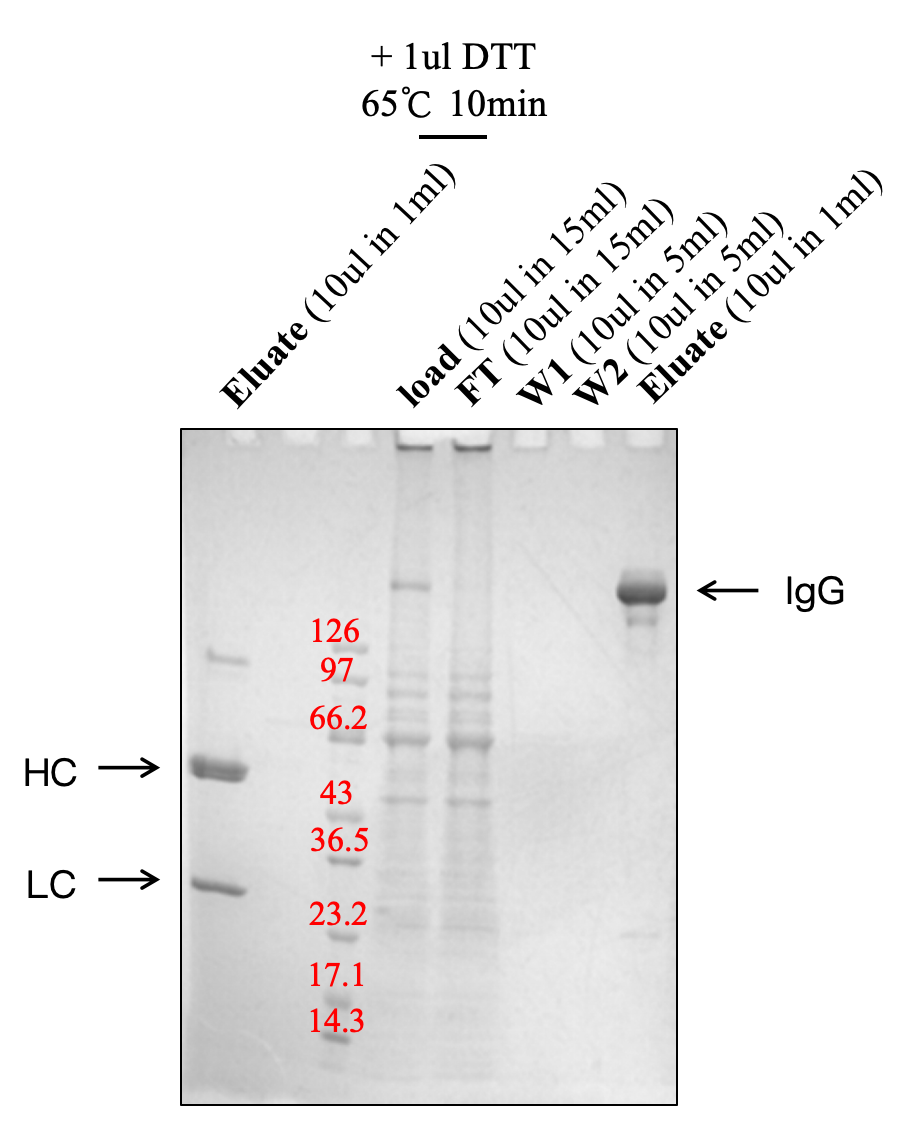
\includegraphics[width=0.4\textwidth]{docs/figures/result/result_05_IgG D4.png}
  \caption{抗HBc IgG的表达与纯化结果。IgG D4在还原条件下显示重链和轻链条带，在非还原条件下显示完整IgG条带，可被用于后续HBV核心蛋白检测。}
  \label{fig:anti-core-igg}
\end{figure}

替换为抗HBc IgG D4后，100 nM preS组与0 nM preS对照组之间的分离度显著改善，尤其是在中高浓度HBVCp149条件下，实验组信号随核心蛋白浓度升高而逐渐增加，而对照组上升较慢。这表明该ELISA模式能够报告一定的preS依赖性核心蛋白结合成分。然而，该体系的动态窗口仍不稳定：绝对信号较低，低浓度点波动明显，不同浓度下计算得到的Z-factor变化较大。最佳Z-factor出现在1280 nM HBVCp149条件下，约为0.397；整体范围为-8.896至0.397，始终未达到通常认为适合稳健筛选的0.5阈值。

\begin{figure}[htb]
  \centering
  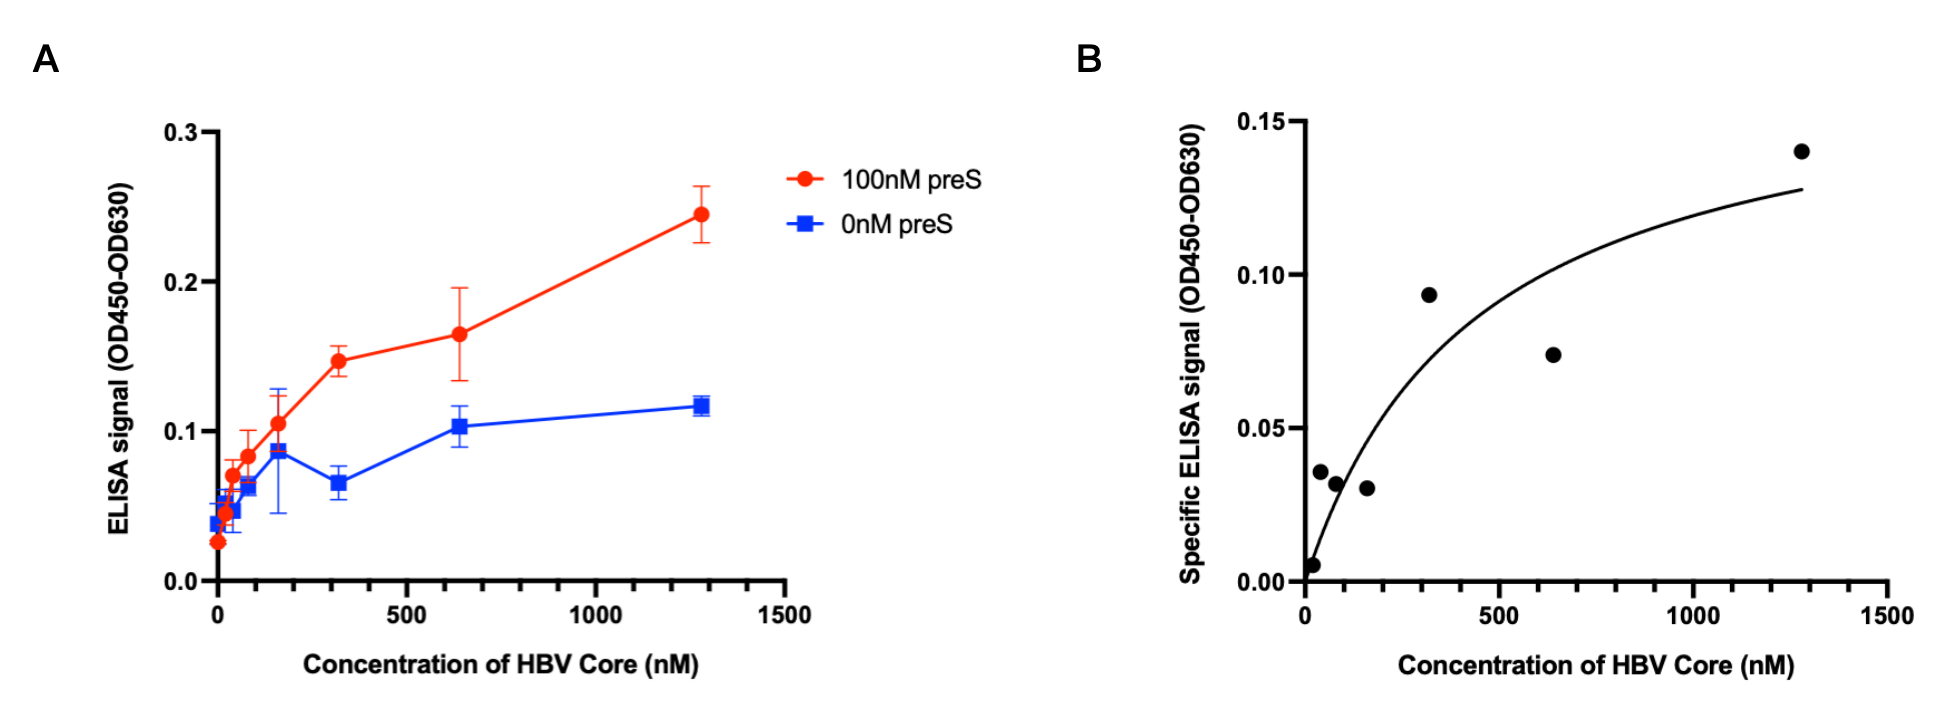
\includegraphics[width=1.0\textwidth]{docs/figures/result/result_06_elisa_b_2.png}
  \caption{替换抗HBc IgG D4后的StrepXT捕获preS的ELISA结果。A，100nM和0nM preS包被后HBc的滴定曲线。B，HBc滴定的特异性信号。中高浓度HBVCp149条件下信噪比显著增加，但Z-factor仍未达到稳健筛选所需水平。}
  \label{fig:elisa-format-b-igg-d4}
\end{figure}

\begin{table}[htbp]
\centering
\caption{StrepXT捕获preS的ELISA模式在不同HBc浓度下的Z-factor}
\label{tab:elisa_b z_factor}
\begin{tabular}{cccccc}
\toprule
浓度 / nM & 实验组均值 & 对照组均值 & 实验组 SD & 对照组 SD & Z - factor \\
\midrule
1280 & 0.1169 & 0.2449 & 0.0067 & 0.0190 & 0.397 \\
640  & 0.1031 & 0.1648 & 0.0138 & 0.0310 & -1.176 \\
320  & 0.0655 & 0.1468 & 0.0112 & 0.0102 & 0.212 \\
160  & 0.0868 & 0.1050 & 0.0416 & 0.0185 & -8.896 \\
80   & 0.0634 & 0.0831 & 0.0062 & 0.0175 & -2.625 \\
40   & 0.0468 & 0.0704 & 0.0144 & 0.0105 & -2.165 \\
20   & 0.0517 & 0.0449 & 0.0093 & 0.0075 & -6.429 \\
0    & 0.0380 & 0.0259 & 0.0136 & 0.0012 & -2.658 \\
\bottomrule
\end{tabular}
\end{table}

因此，StrepXT捕获preS体系虽然较直接包被体系有所改进，但仍不足以作为后续系统比较preS突变体或小分子抑制效果的主要平台。该结果提示，在preS呈递已得到改善后，限制体系表现的主要因素可能转移为核心蛋白检测灵敏度、固相体系中的结合稳定性以及洗涤过程导致的弱相互作用解离。

\subsection{ELISA模式三：抗HBc Fab捕获HBc}

第三种ELISA构型尝试从核心蛋白呈递方式入手进行优化。该体系首先利用抗HBc Fab捕获HBVCp149，再加入preS，并通过抗GST抗体检测preS信号。与HBc直接吸附于塑料表面相比，抗体介导捕获理论上更有利于保留HBc颗粒构象，并减少核心蛋白表面互作位点被随机吸附遮挡的可能性。

核心蛋白滴定结果显示，50 nM抗HBc Fab能够有效捕获HBVCp149，且信号随核心蛋白浓度升高逐渐接近饱和，说明捕获步骤本身在技术上可行。随后在固定HBc条件下进行preS滴定，实验组信号随preS浓度增加而升高，说明体系中可以检测到preS相关读数。然而，未加入HBc的对照组信号也出现明显升高，且二抗HRP-only对照不能完全解释这一背景来源。扣除背景后，50 nM HBc组与0 nM HBc组之间的特异信号差异仍然较小，整体窗口未能明显扩大。

\begin{figure}[htbp]
  \centering
  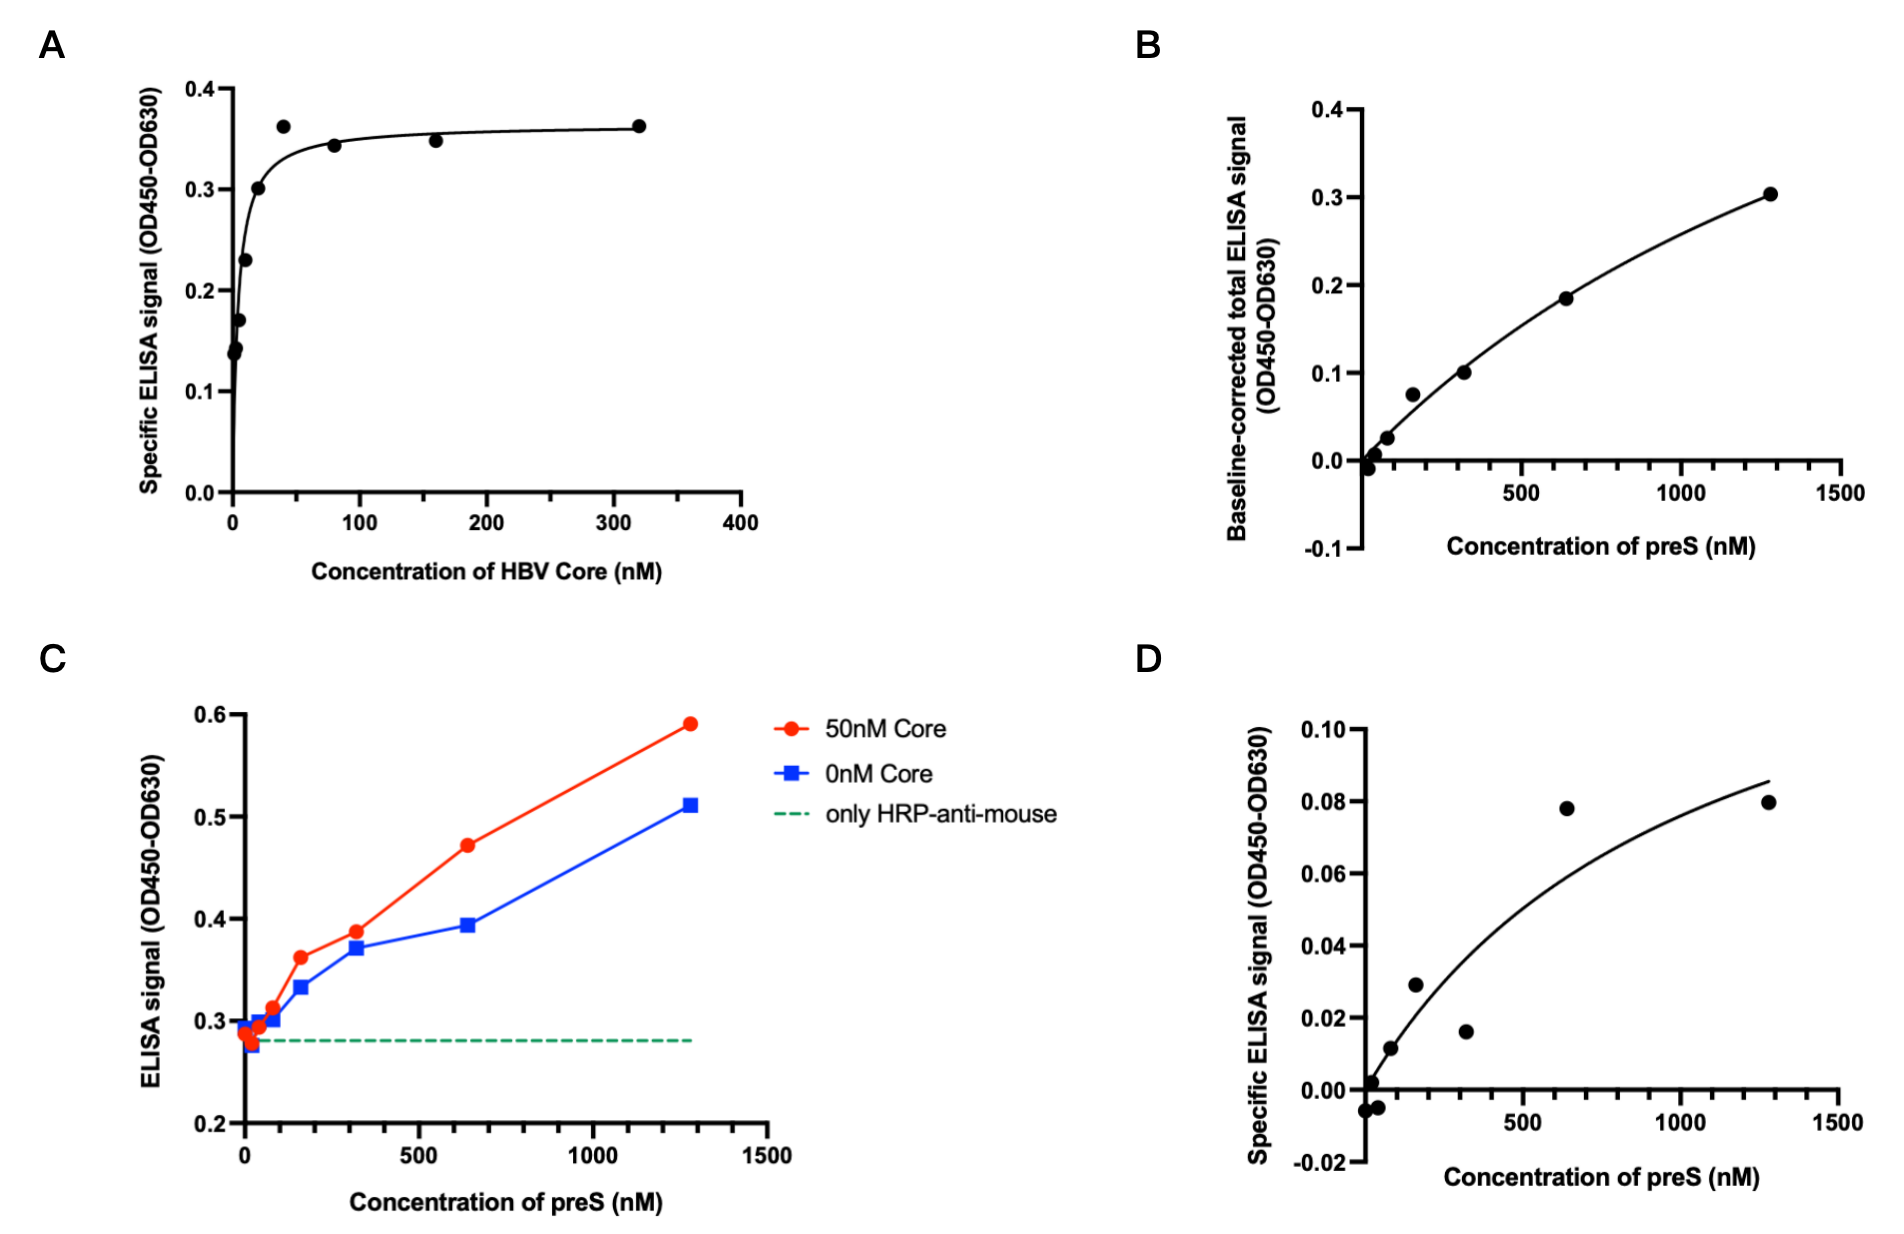
\includegraphics[width=1.0\textwidth]{docs/figures/result/result_07_elisa_c.png}
  \caption{抗HBc Fab捕获HBc的ELISA模式的检测结果。A，抗HBc Fab能够捕获HBVCp149并产生可饱和信号。B、C、D，preS滴定中无HBc对照仍出现明显背景，导致特异窗口较窄，无法作为有效的检测手段。}
  \label{fig:elisa-format-c}
\end{figure}

这一结果说明，即便通过抗core Fab捕获方式改善HBc固定化，ELISA体系仍难以获得干净且稳定的preS依赖性读数。可能原因包括preS或抗GST抗体仍存在非特异吸附，HBc被捕获后的空间取向不一定有利于preS结合，以及HBc--preS相互作用本身较弱、容易在洗涤过程中解离。

\subsection{三种ELISA体系的综合分析}

综合三种ELISA构型可以看出，它们分别受限于不同步骤，但共同指向同一结论：常规固相ELISA并不适合作为HBc--preS弱相互作用的主要下游定量平台。HBc直接包被体系主要受preS和抗体非特异吸附影响；StrepXT捕获preS体系改善了preS呈递，但核心蛋白检测窗口仍不足；抗HBc Fab捕获HBc体系改善了核心蛋白固定方式，却仍未能显著降低preS检测背景。

这些结果提示，体外HBc--preS相互作用可能具有亲和力较弱、构象依赖性强和多价效应敏感等特点。ELISA依赖蛋白固定化、多步孵育和反复洗涤，容易破坏弱相互作用平衡，也可能因固相表面吸附而放大背景信号。尤其对于后续需要比较不同preS突变体和不同小分子抑制条件的实验，检测平台不仅需要能够区分实验组与阴性对照，还需要具有足够稳定的动态范围和统计学鲁棒性。从目前结果看，ELISA最多可作为辅助验证手段，而不适合作为主要筛选和定量比较平台。

\section{NanoBiT检测体系的建立、优化与应用}

\subsection{NanoBiT相关融合蛋白的构建与试表达}

基于ELISA体系的局限，本研究进一步转向NanoBiT发光互补体系。该体系不依赖反复洗涤，而是在接近溶液状态的条件下检测两个融合蛋白之间的空间接近，因此更适合检测弱而可逆的蛋白相互作用。考虑到较大的LgBiT可能影响HBc组装，本研究将较小的SmBiT融合至HBVCp182，而将LgBiT融合至含preS 87--114片段的GST融合蛋白。同时设置不含preS的LgBiT融合蛋白作为阴性对照，并利用GST标签的二聚化特性设置阳性对照，从而在同一体系内比较特异互作、非特异互补和检测上限。

\begin{figure}[htbp]
  \centering
  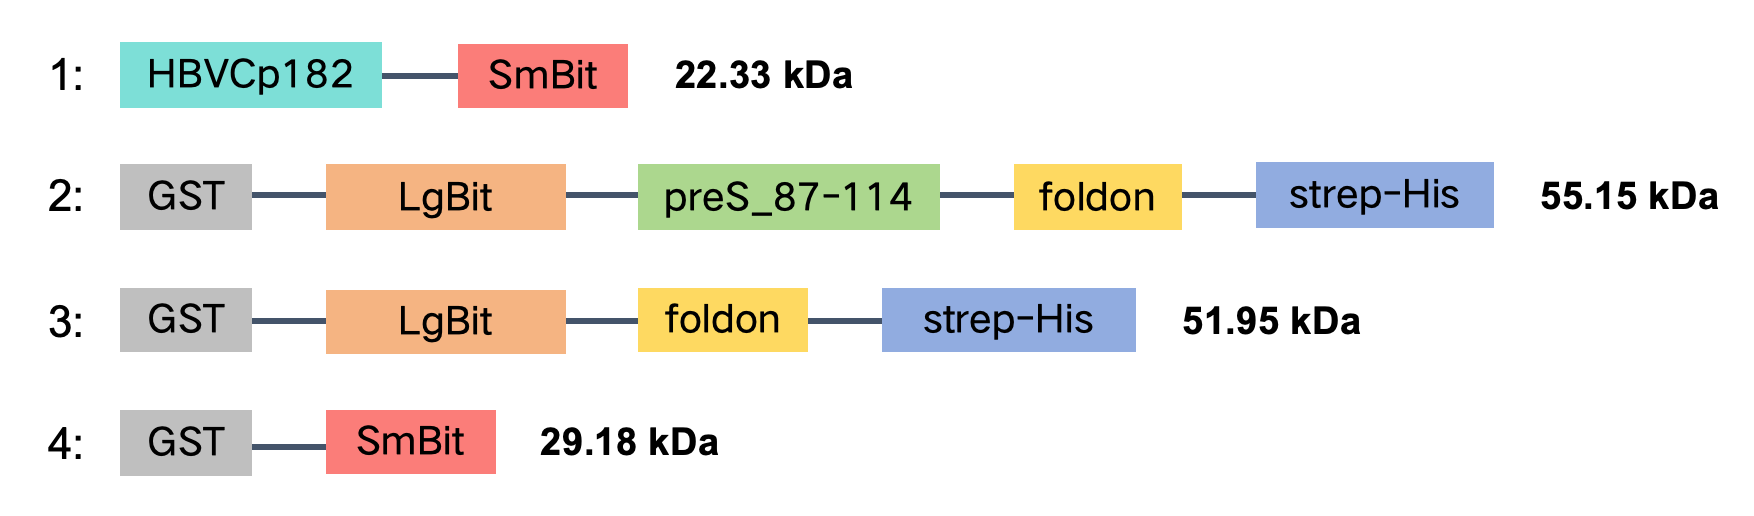
\includegraphics[width=1.0\textwidth]{docs/figures/result/result_08_constructs_ljq_1234.png}
  \caption{NanoBiT相关融合蛋白的构建}
  \label{fig:nanobit-constructs-1234}
\end{figure}

首先对NanoBiT相关构建体进行了小规模表达检测。结果显示，在测试条件下，四种融合蛋白均可检测到表达，其中一组诱导条件下目标蛋白表达较为明显，因此被选为后续蛋白制备的参考条件。随后对HBVCp182-SmBiT进行盐析和SP柱纯化，目标条带能够在洗脱组分中检测到，但纯度仍不理想，说明该蛋白制备流程仍需进一步优化。相比之下，GST标记的LgBiT融合蛋白以及GST-SmBiT均能够成功表达并通过GST亲和纯化获得较明显的目标条带，表明NanoBiT实验所需的preS融合蛋白、阴性对照和阳性对照在技术上均可获得。

\begin{figure}[htbp]
  \centering
  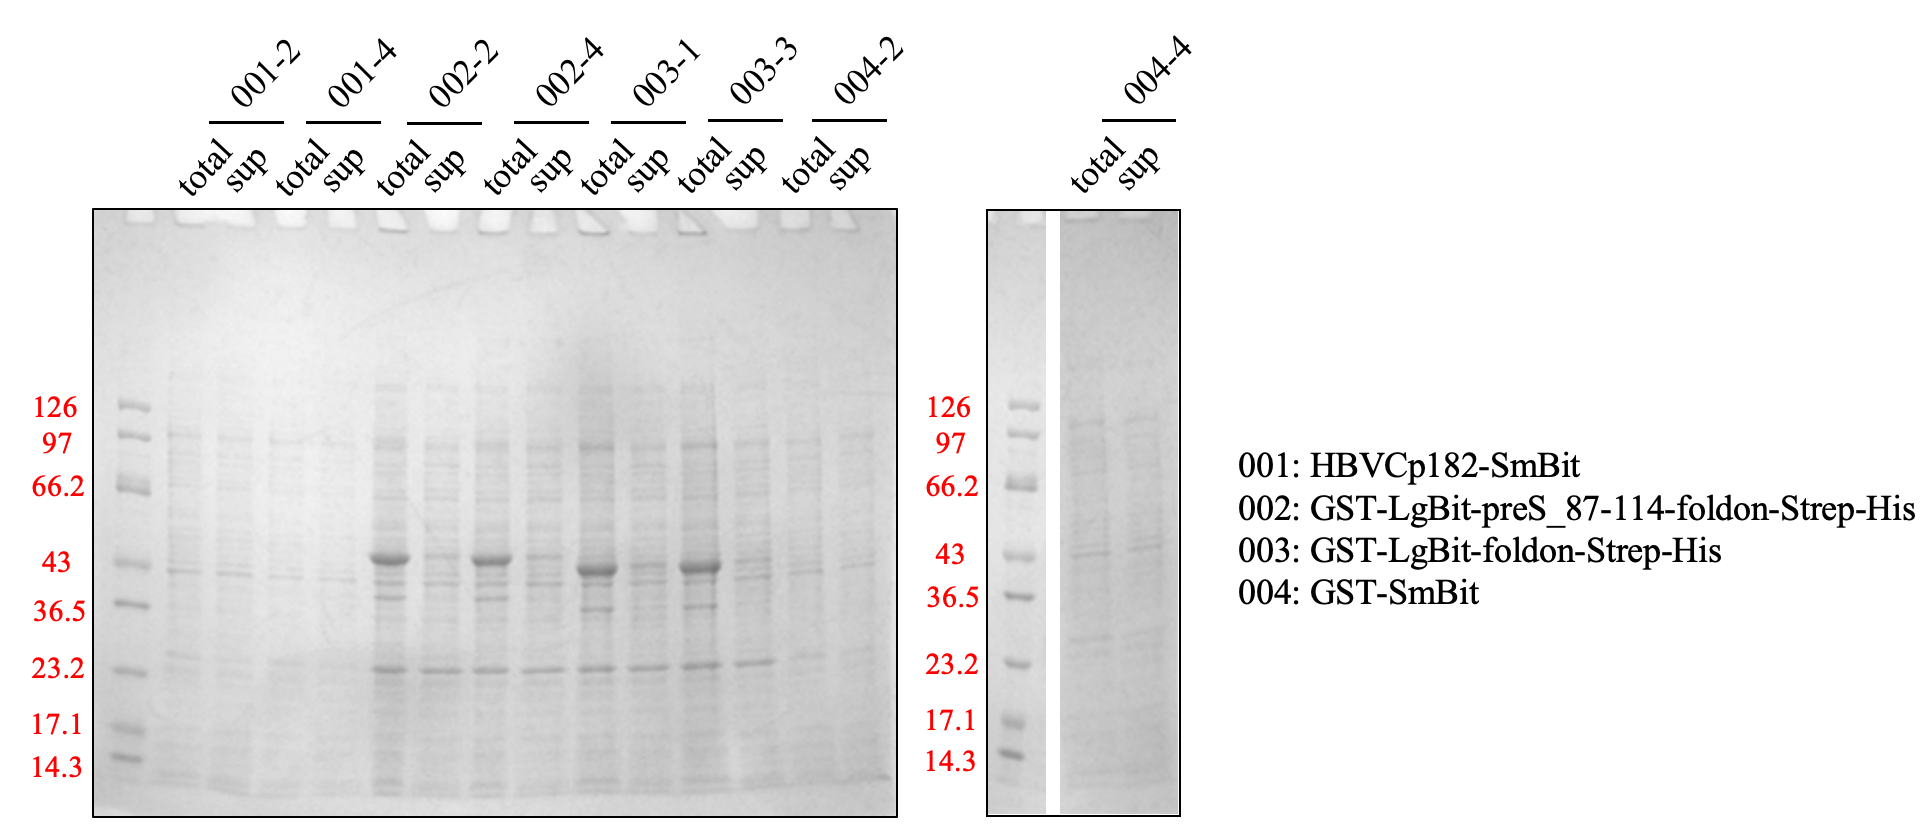
\includegraphics[width=0.9\textwidth]{docs/figures/result/result_09_expression_test_ljq_1234.png}
  \caption{NanoBiT相关构建体的小规模表达检测。四种融合蛋白在测试条件下均可检测到表达，为后续纯化和发光互补实验提供了基础。}
  \label{fig:nanobit-expression-test}
\end{figure}

\subsection{HBVCp182-SmBit的表达纯化与活性检测}

将HBVCp182-SmBiT的重组质粒转入NiCo21大肠杆菌并在37°C诱导表达4小时后，经分步盐析与Q HP阴离子交换层析，在层析图谱上显示多个紫外吸收峰，其中约15.01 mL、18.68 mL和24.80 mL附近的峰与后续SDS-PAGE和Western blot检测中的目标蛋白分布相对应。

SDS-PAGE结果显示，HBVCp182-SmBiT目标条带位于约22.33 kDa附近，并在Q柱洗脱组分中明显富集。进一步使用anti-HBcAg抗体进行Western blot检测时，相同组分出现明确的HBc相关条带，确认该条带对应HBVCp182-SmBiT。基于电泳、免疫印迹和后续活性检测结果，将Q柱9--13管和15--22管分别合并，用于进一步比较其NanoBiT检测活性。

\begin{figure}[htbp]
  \centering
  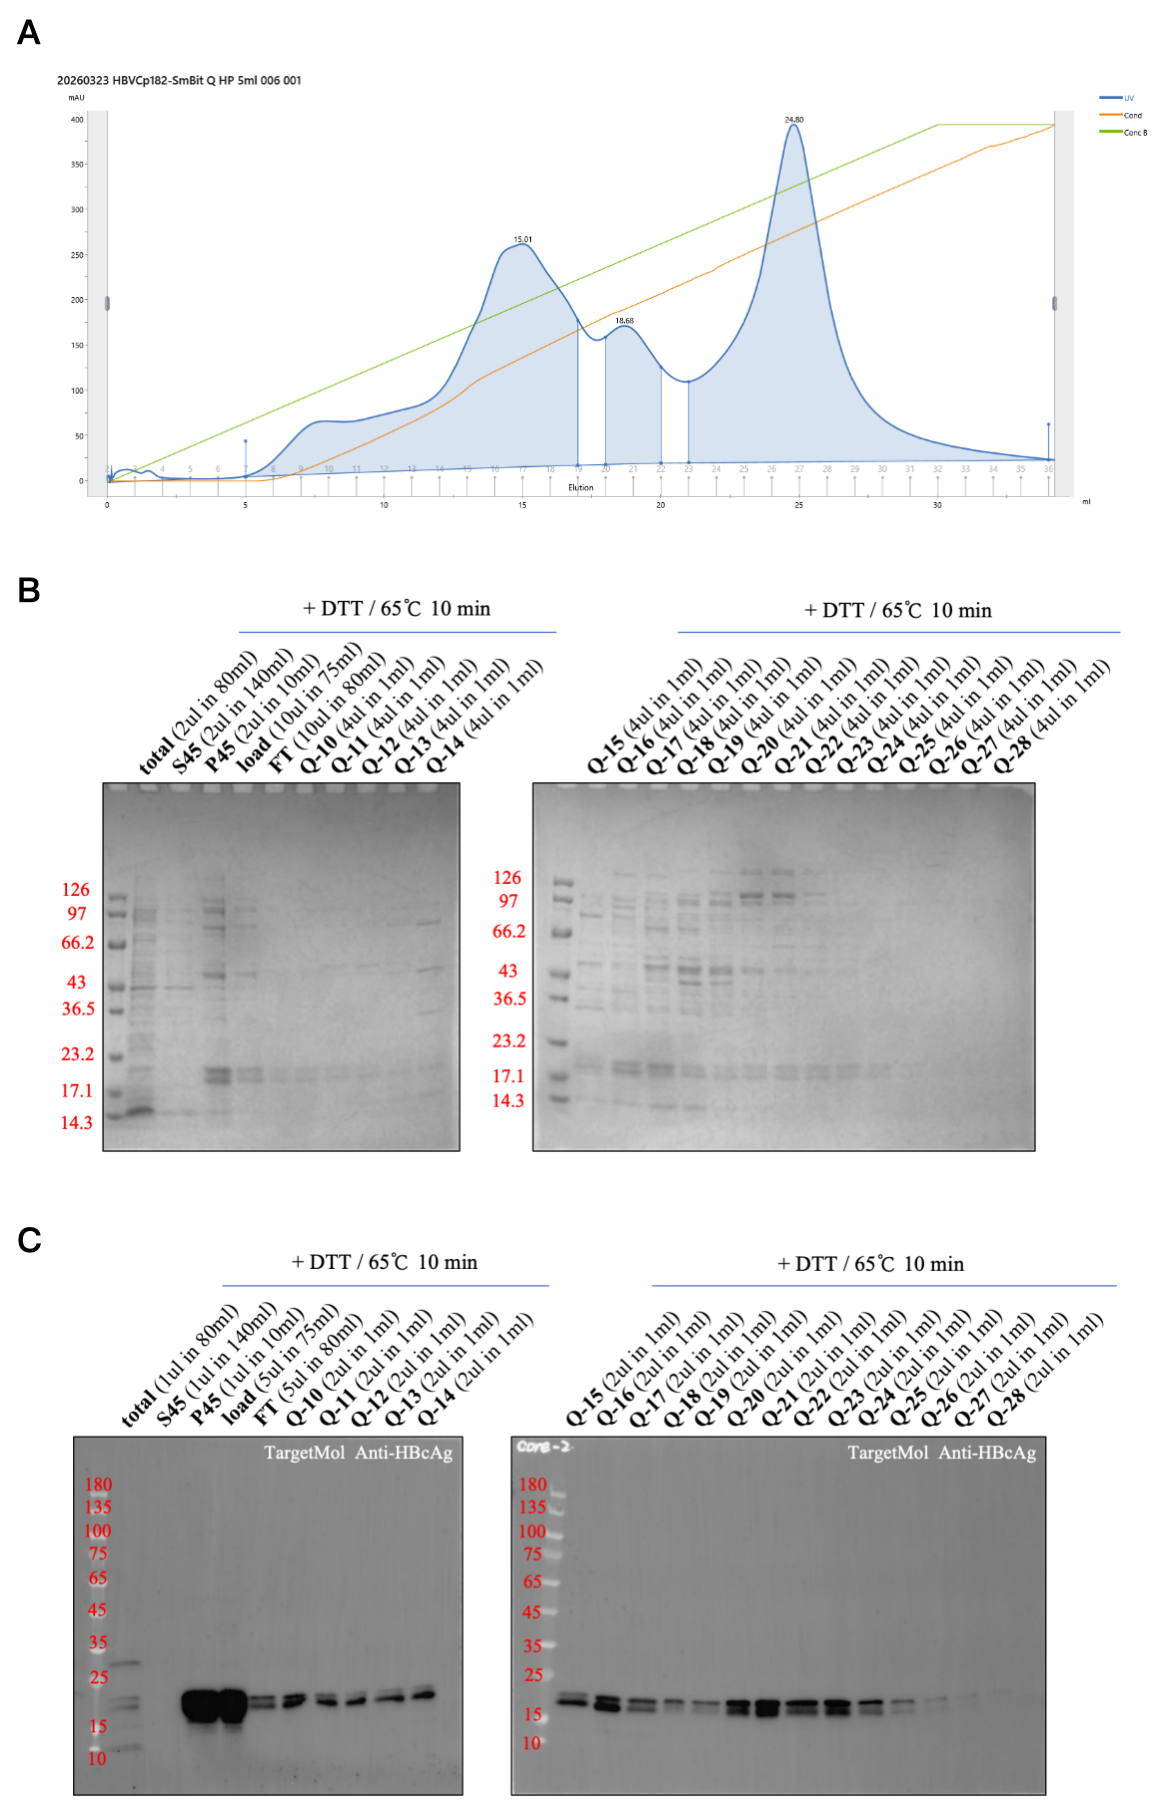
\includegraphics[width=1.0\textwidth]{docs/figures/result/result_10_ljq_1.png}
  \caption{HBVCp182-SmBiT的表达与纯化结果。目标蛋白可在洗脱组分中检测到.}
  \label{fig:hbvcp182-smbit-purification}
\end{figure}

为判断不同Q柱合并组分是否具有相近功能活性，分别使用Q 9--13和Q 15--22两组合并样品进行NanoBiT检测。两组合并组分均产生明显高于阴性对照和HBc-only背景的发光信号，说明重新纯化后的HBVCp182-SmBiT保留了检测preS结合的功能。Q 9--13组分实验组平均信号为1644.00 RLU，阴性对照为289.67 RLU，特异性窗口约为1354.33 RLU；Q 15--22组分实验组平均信号为1875.00 RLU，阴性对照为245.67 RLU，特异性窗口约为1629.33 RLU。Q 15--22组分信号略高，但两组合并组分均可支持后续实验。基于蛋白利用率和批次一致性考虑，后续将两组合并作为后续NanoBiT实验中的核心蛋白来源。

\begin{table}[htbp]
  \centering
  \caption{不同Q柱合并组分NanoBiT活性检测}
  \label{tab:NanoBiT-test-data}
  \begin{tabular}{cccc}
    \toprule
    & \makecell{80 nM GST-LgBit-preS\\ 实验组} & \makecell{80 nM GST-LgBit\\ 阴性对照} & 
    \makecell{only HBVCp182-SmBit\\ 空白对照} \\
    \midrule
    \multirow{3}{*}{Q 9-13}  & 1679 & 297 & 51 \\
                             & 1782 & 305 & 31 \\
                             & 1471 & 267 & 33 \\
    \midrule
    \multirow{3}{*}{Q 15-22} & 2102 & 211 & 37 \\
                             & 1804 & 283 & 16 \\
                             & 1719 & 243 & 25 \\
    \bottomrule
  \end{tabular}
\end{table}

\begin{figure}[htbp]
  \centering
  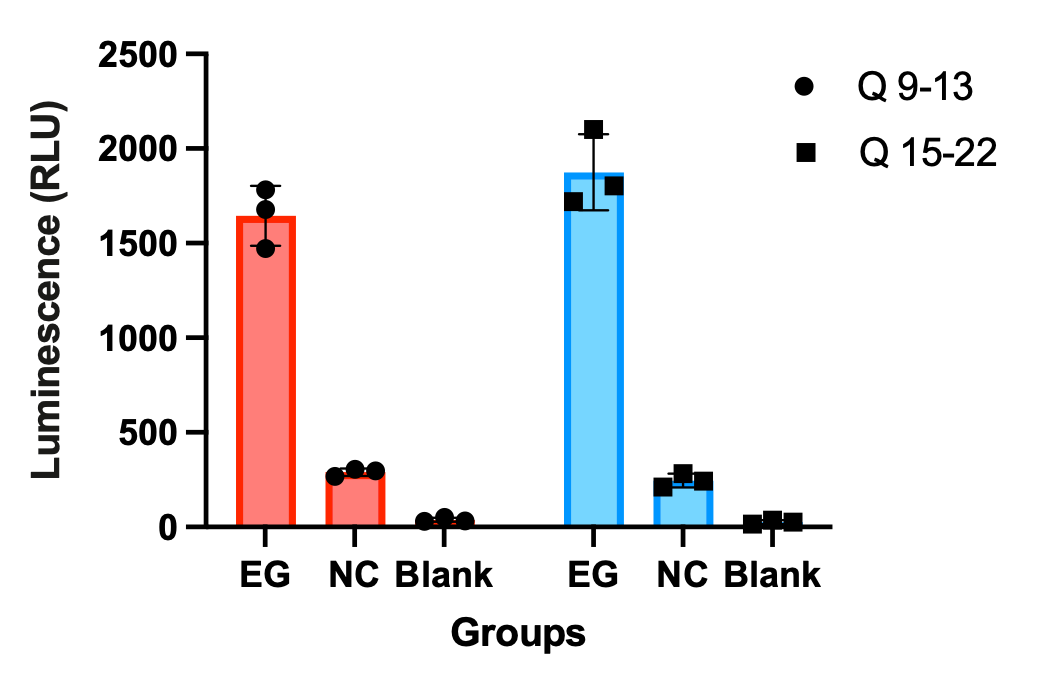
\includegraphics[width=0.7\textwidth]{docs/figures/result/result_11_nanobit_test.png}
  \caption{Q 9--13和Q 15--22两组合并HBVCp182-SmBiT样品的NanoBiT活性比较。两组均显示出显著高于阴性对照和HBc-only背景的发光信号。}
  \label{fig:hbvcp182-smbit-q-fraction-activity}
\end{figure}

\subsection{三种GST标签融合蛋白的表达与纯化}

两种GST标签的LgBiT融合蛋白及GST-SmBiT均成功表达并纯化，在GST洗脱组分中可观察到明确的目的条带。该结果表明，实验组以及阳性、阴性对照所需的NanoBiT体系各组成元件均已成功获得，从而为在同一检测体系中比较特异性与非特异性互补信号提供了实验基础。

\begin{figure}[htbp]
  \centering
  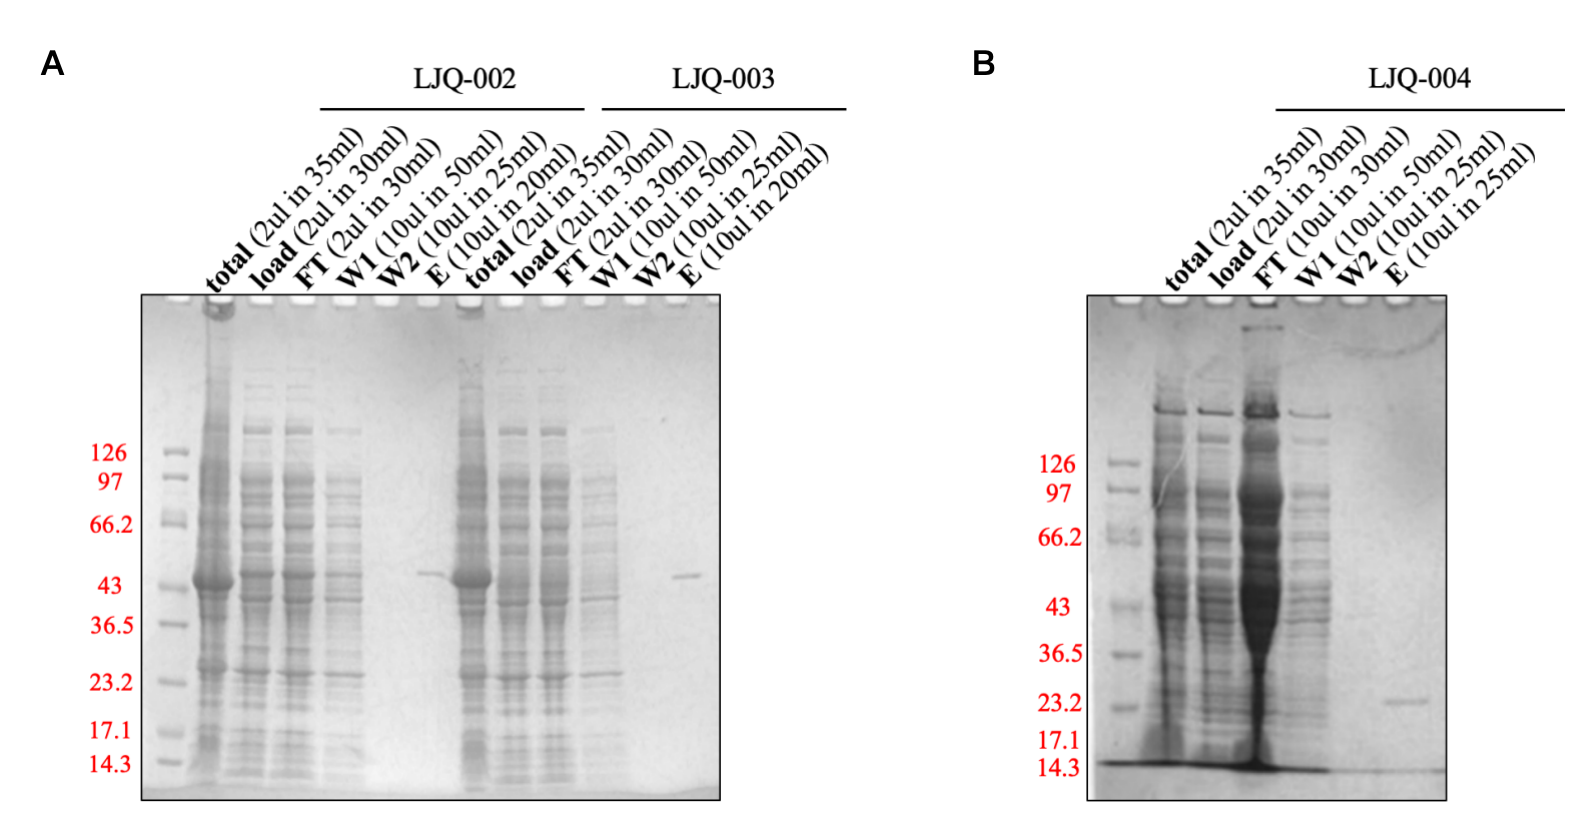
\includegraphics[width=0.95\textwidth]{docs/figures/result/result_12_ljq_234.png}
  \caption{三种GST标签融合蛋白的表达纯化结果。A，GST-LgBiT-preS（002）及GST-LgBiT（003）经GST层析柱后各组分的SDS-PAGE分析。B，GST-SmBiT（004）经GST层析柱后各组分的SDS-PAGE分析。相关对照蛋白和preS融合蛋白均可获得，为NanoBiT互作检测提供了实验材料。}
  \label{fig:gst-lgbit-purification}
\end{figure}

\subsection{NanoBiT体系的初步发光检测}

在初步发光检测中，将LgBiT融合蛋白与SmBiT融合蛋白按1:1浓度比例混合，结果显示HBVCp182-SmBiT与含preS 87--114的LgBiT融合蛋白组合产生的发光信号持续高于阴性对照。与此同时，GST介导的阳性对照产生最高信号，说明NanoBiT报告系统本身具有可检测的上限窗口；仅含单一融合蛋白的孔接近基线，提示LgBiT和SmBiT自发互补造成的背景较低。该结果说明，NanoBiT体系能够将HBc与preS片段之间的接近事件转化为可检测的发光信号。

\begin{figure}[htbp]
  \centering
  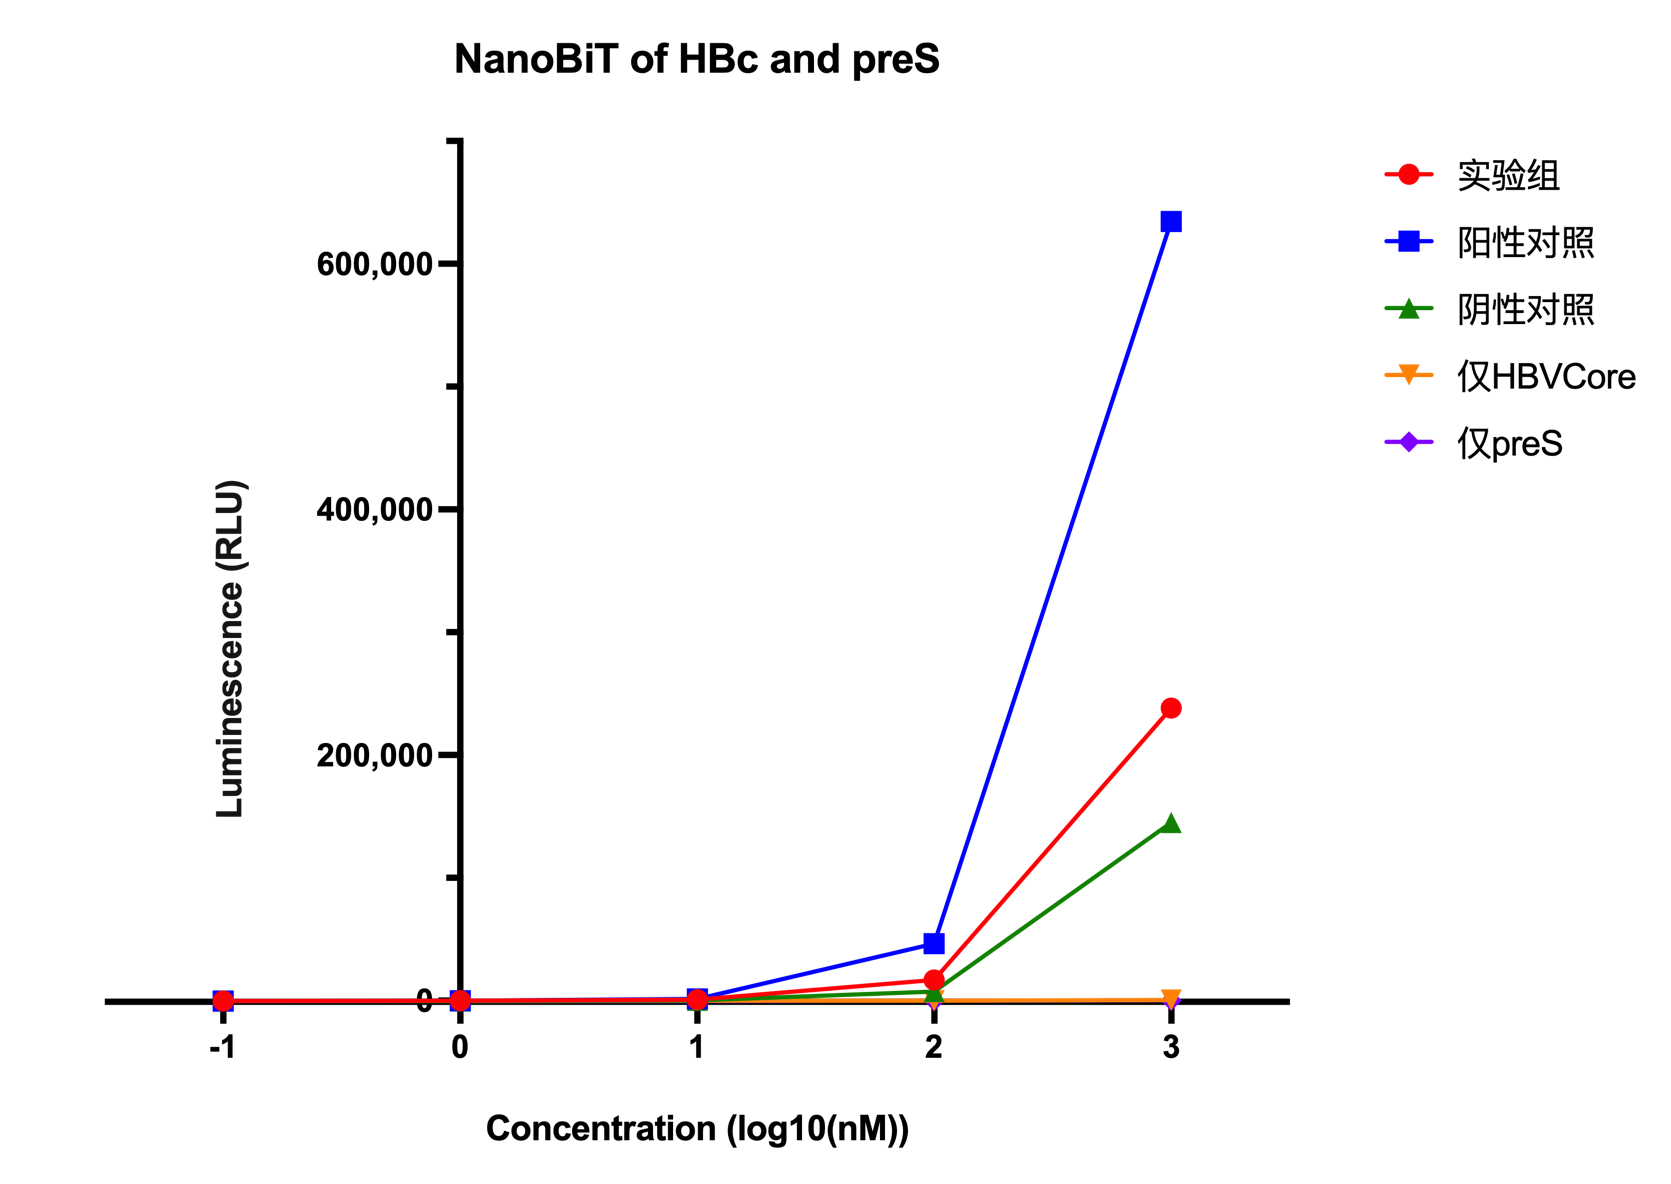
\includegraphics[width=0.62\textwidth]{figures/result/result_31.png}
  \caption{NanoBiT体系1:1浓度比例下的初步检测结果。HBVCp182-SmBiT与preS 87--114-LgBiT组合的发光信号高于阴性对照，阳性对照显示检测体系具有足够的信号上限。}
  \label{fig:nanobit-one-to-one}
\end{figure}

进一步固定HBVCp182-SmBiT浓度为50 nM并滴定含preS 87--114的LgBiT融合蛋白时，实验组与阴性对照之间的分离随LgBiT-preS浓度升高而逐渐增强。实验组总发光信号呈浓度依赖性上升，扣除背景后的特异信号呈现趋于饱和的趋势，符合有限互作复合物形成的特征。定量结果显示，当LgBiT-preS终浓度为40、80和160 nM时，实验组发光信号分别约为3295.33、4873.67和7194.67 RLU，而对应阴性对照分别约为915.67、1561.67和2697.67 RLU。相应Z-factor分别为0.608、0.695和0.623，均超过0.5；20 nM条件下Z-factor约为0.485，处于临界范围。

\begin{figure}[htbp]
  \centering
  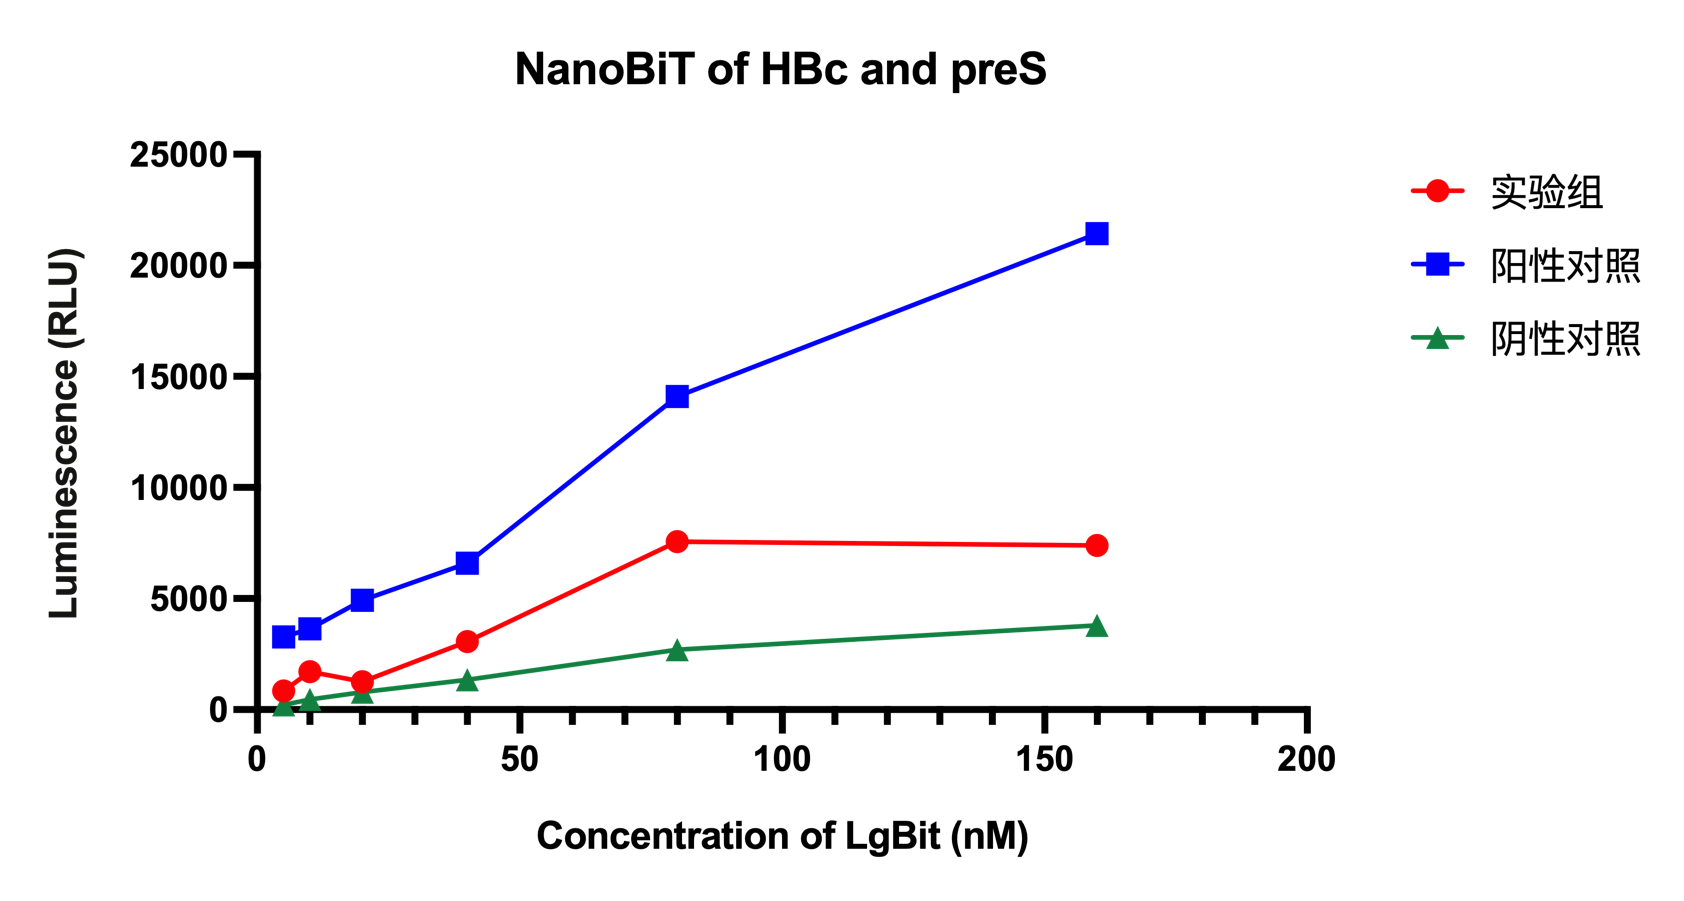
\includegraphics[width=0.46\textwidth]{figures/result/result_32.png}
  \hfill
  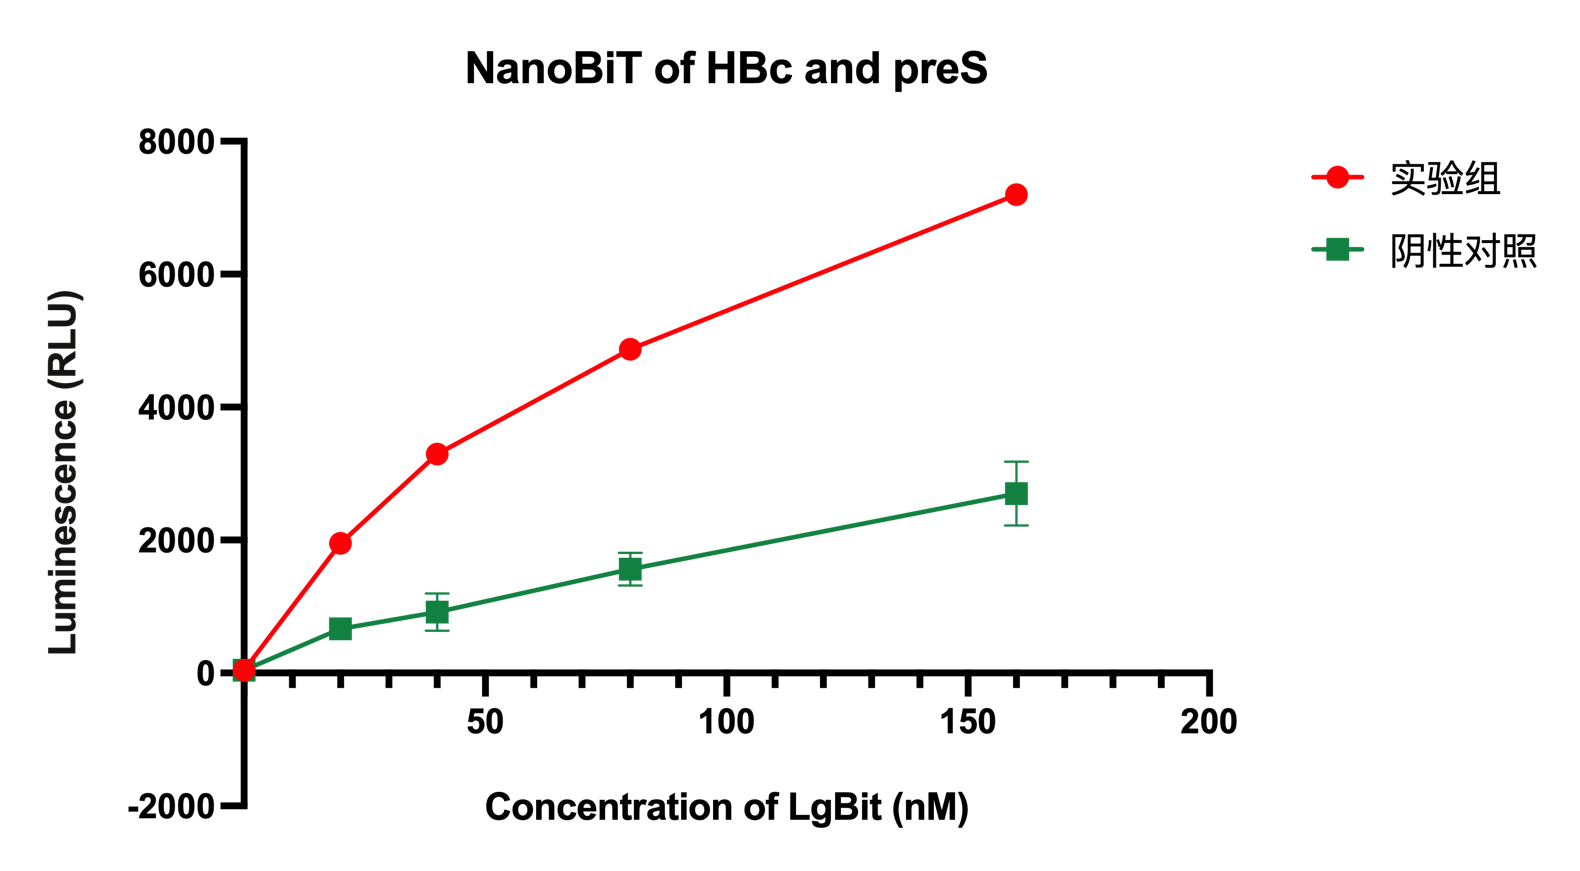
\includegraphics[width=0.46\textwidth]{figures/result/result_33.png}
  \par\medskip
  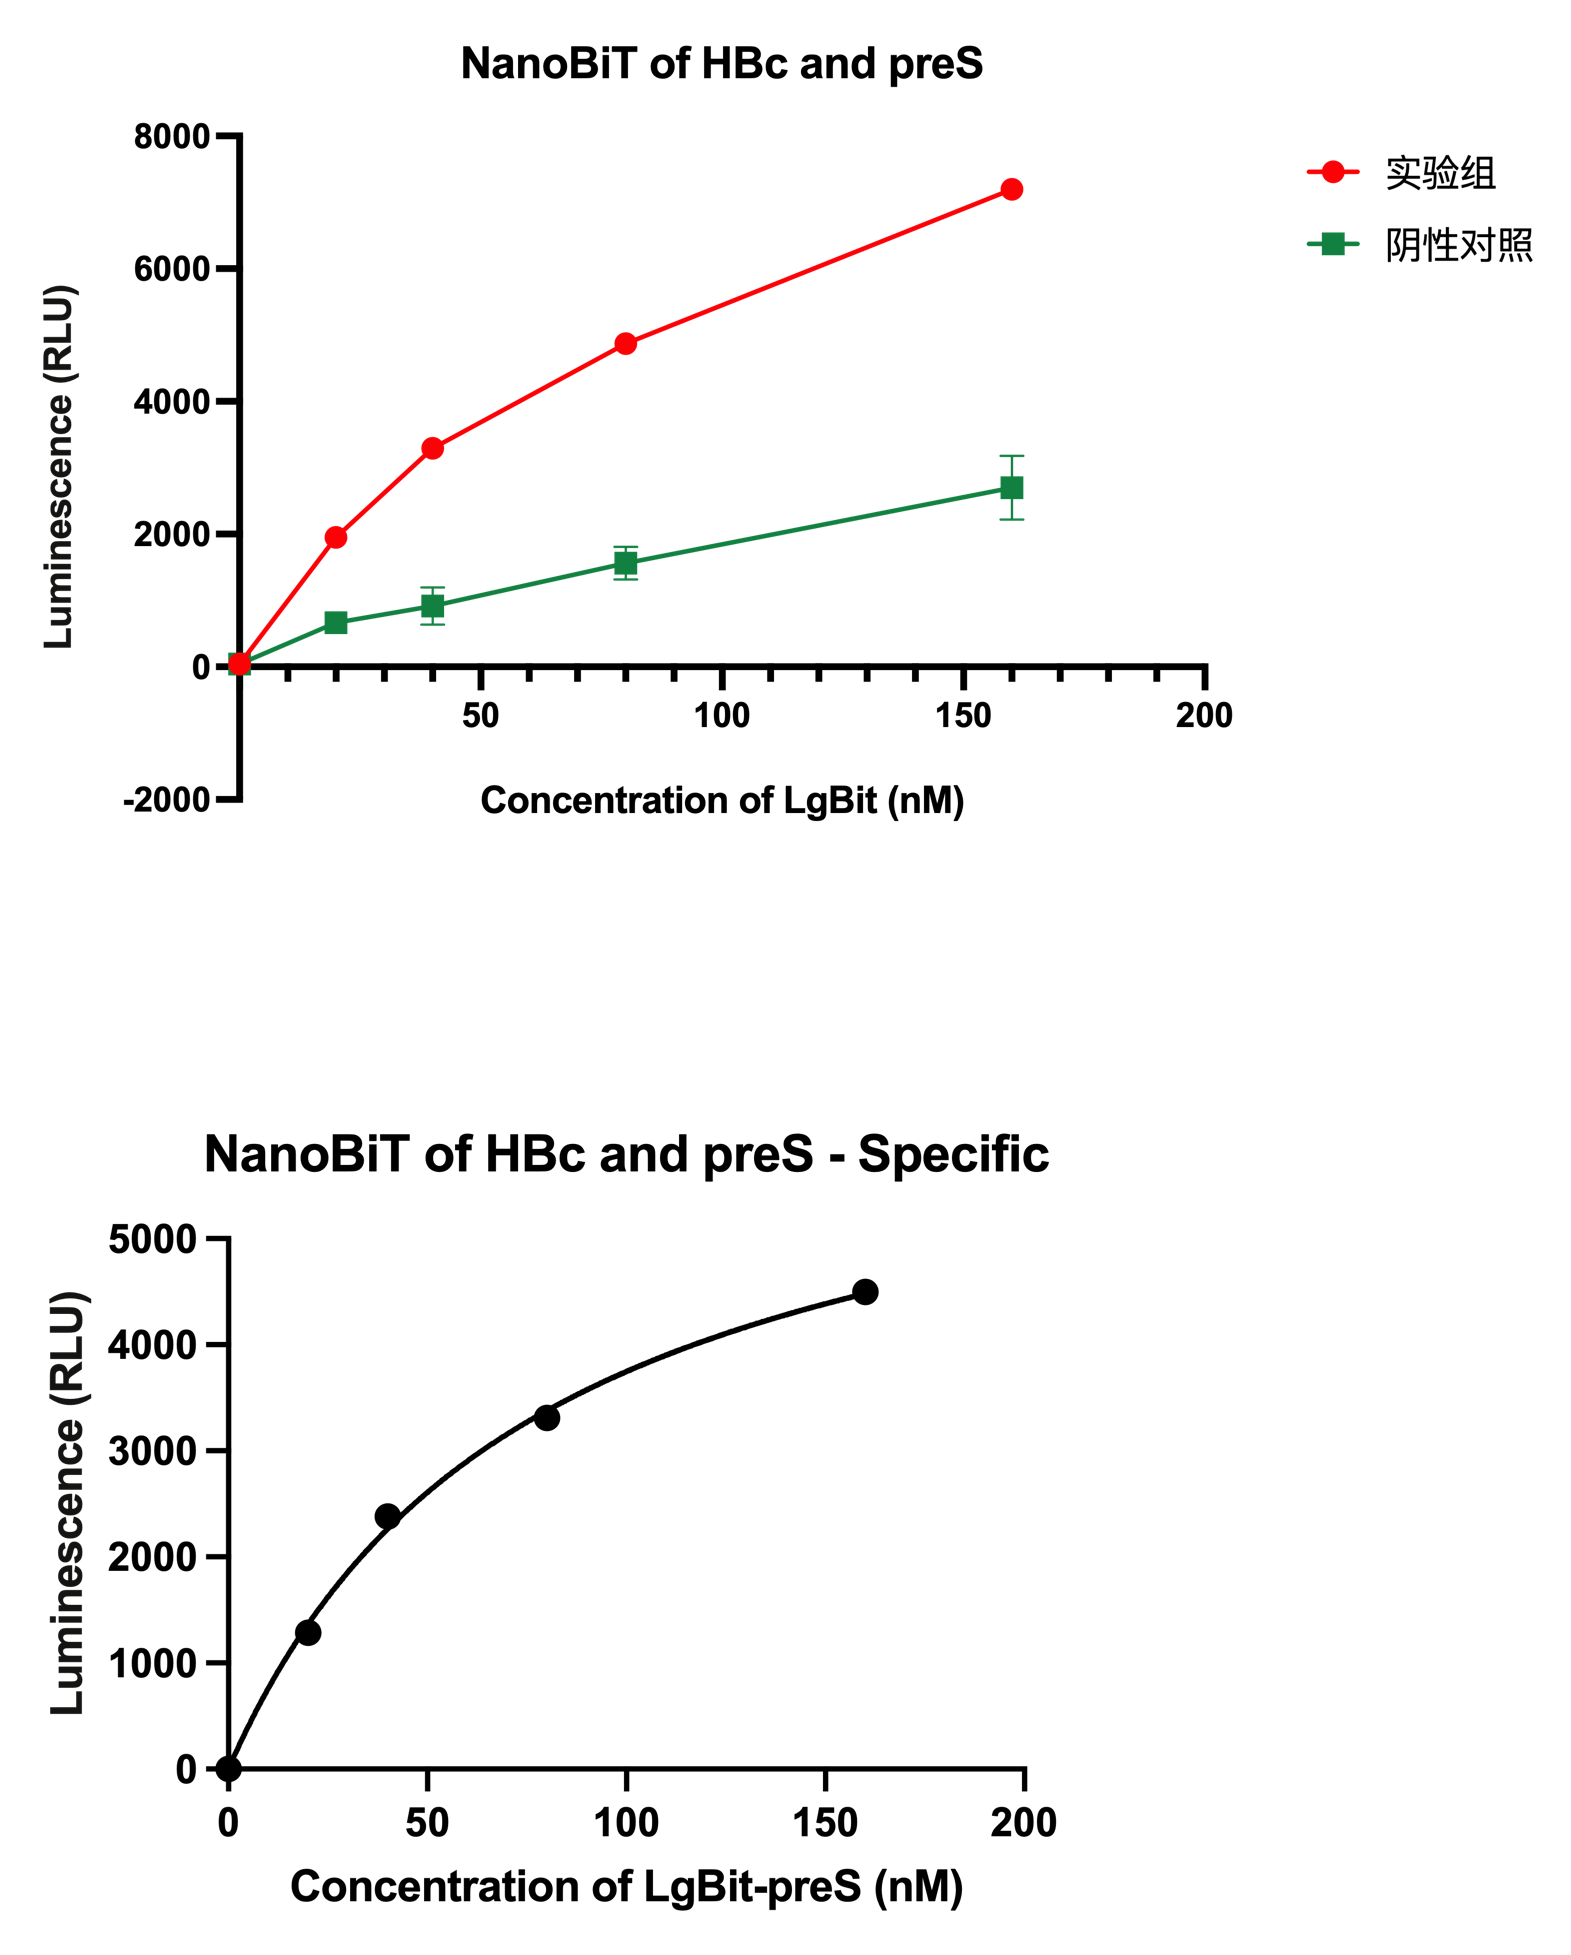
\includegraphics[width=0.35\textwidth]{figures/result/result_34.png}
  \hfill
  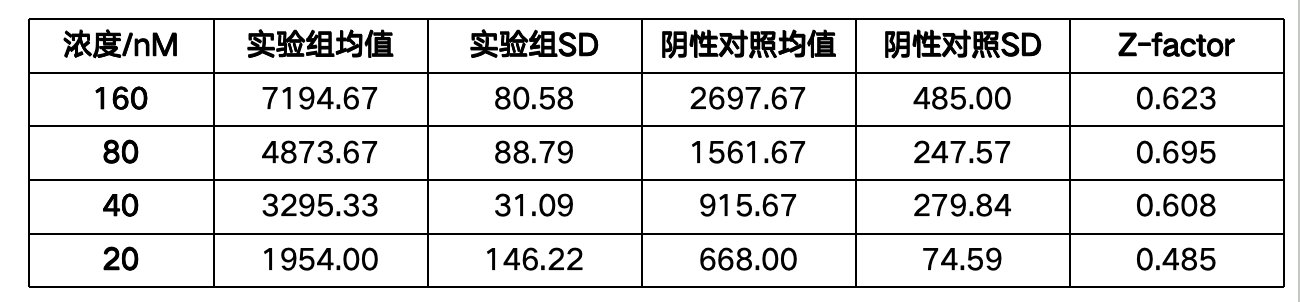
\includegraphics[width=0.55\textwidth]{figures/result/result_35.png}
  \caption{固定HBVCp182-SmBiT浓度后的NanoBiT滴定结果。随着preS 87--114-LgBiT浓度升高，实验组与阴性对照逐渐分离，部分条件下Z-factor超过0.5，显示该体系具备后续定量比较的可行性。}
  \label{fig:nanobit-fixed-core}
\end{figure}

上述结果表明，在合适蛋白浓度条件下，NanoBiT体系能够提供比ELISA更稳定的实验组--阴性对照分离度和更好的统计学窗口。尤其当LgBiT-preS浓度达到40 nM及以上时，该体系已具备进行后续定量比较的基础。结合ELISA结果，可以认为NanoBiT更适合作为本研究后续分析preS关键突变体和小分子抑制作用的主要检测平台。

\subsection{新纯化HBVCp182-SmBiT重复NanoBiT滴定实验}

使用合并后的新纯化HBVCp182-SmBiT进一步重复HBc与preS 87--114相互作用的NanoBiT浓度梯度实验。结果显示，随着GST-LgBiT-preS 87--114融合蛋白浓度升高，实验组发光信号持续增加；阴性对照虽然也随蛋白浓度升高而升高，但始终明显低于实验组。扣除阴性对照后的特异性信号呈现趋于饱和的曲线形态，说明该体系主要报告有限的HBc--preS相互作用，而不是无上限的非特异性NanoLuc片段互补。

定量结果显示，在10--640 nM LgBiT-preS范围内，实验组平均信号由939.00 RLU增加至11320.67 RLU，阴性对照由93.00 RLU增加至4691.67 RLU，特异性信号由846.00 RLU增加至6629.00 RLU。10、20、160和320 nM条件下的Z-factor均高于0.5，其中20 nM和320 nM分别达到0.859和0.770，说明这些浓度下实验组和阴性对照具有较好统计分离度。40、80和640 nM条件下Z-factor低于0.5，主要可能与实验组变异或高浓度背景升高有关。尽管80 nM条件的Z-factor为0.403，但该条件下实验组信号明显高于背景，曲线仍处于较敏感的上升区间，且蛋白消耗低于更高浓度条件，因此被选为含foldon体系下小分子初筛的工作浓度。

\begin{figure}[htbp]
  \centering
  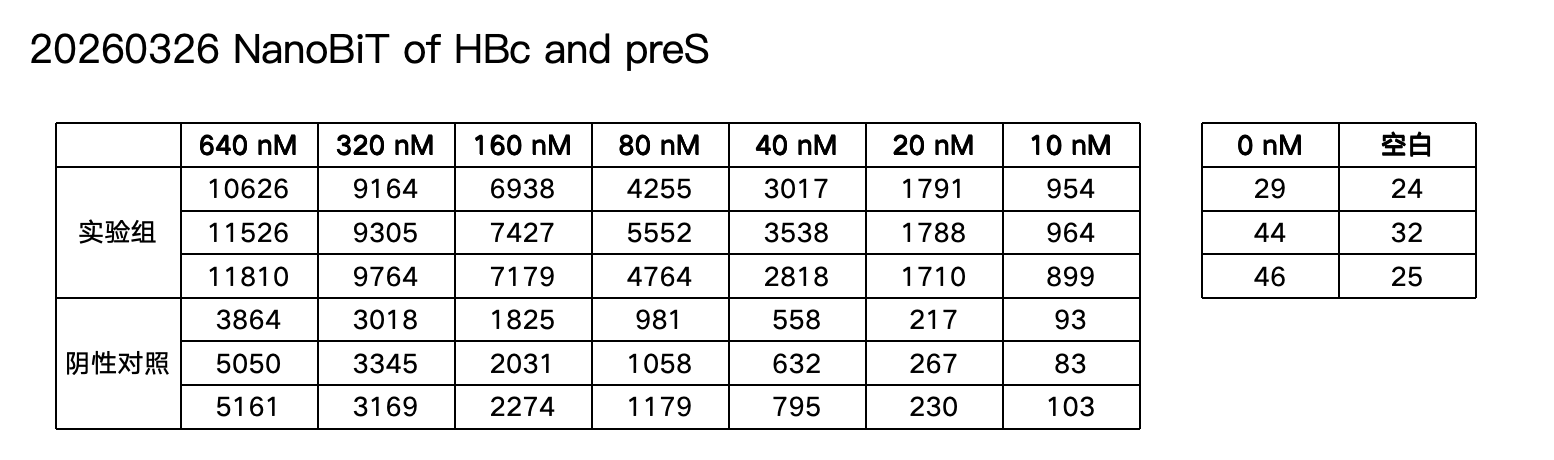
\includegraphics[width=0.82\textwidth]{figures/result/result_40.png}
  \par\medskip
  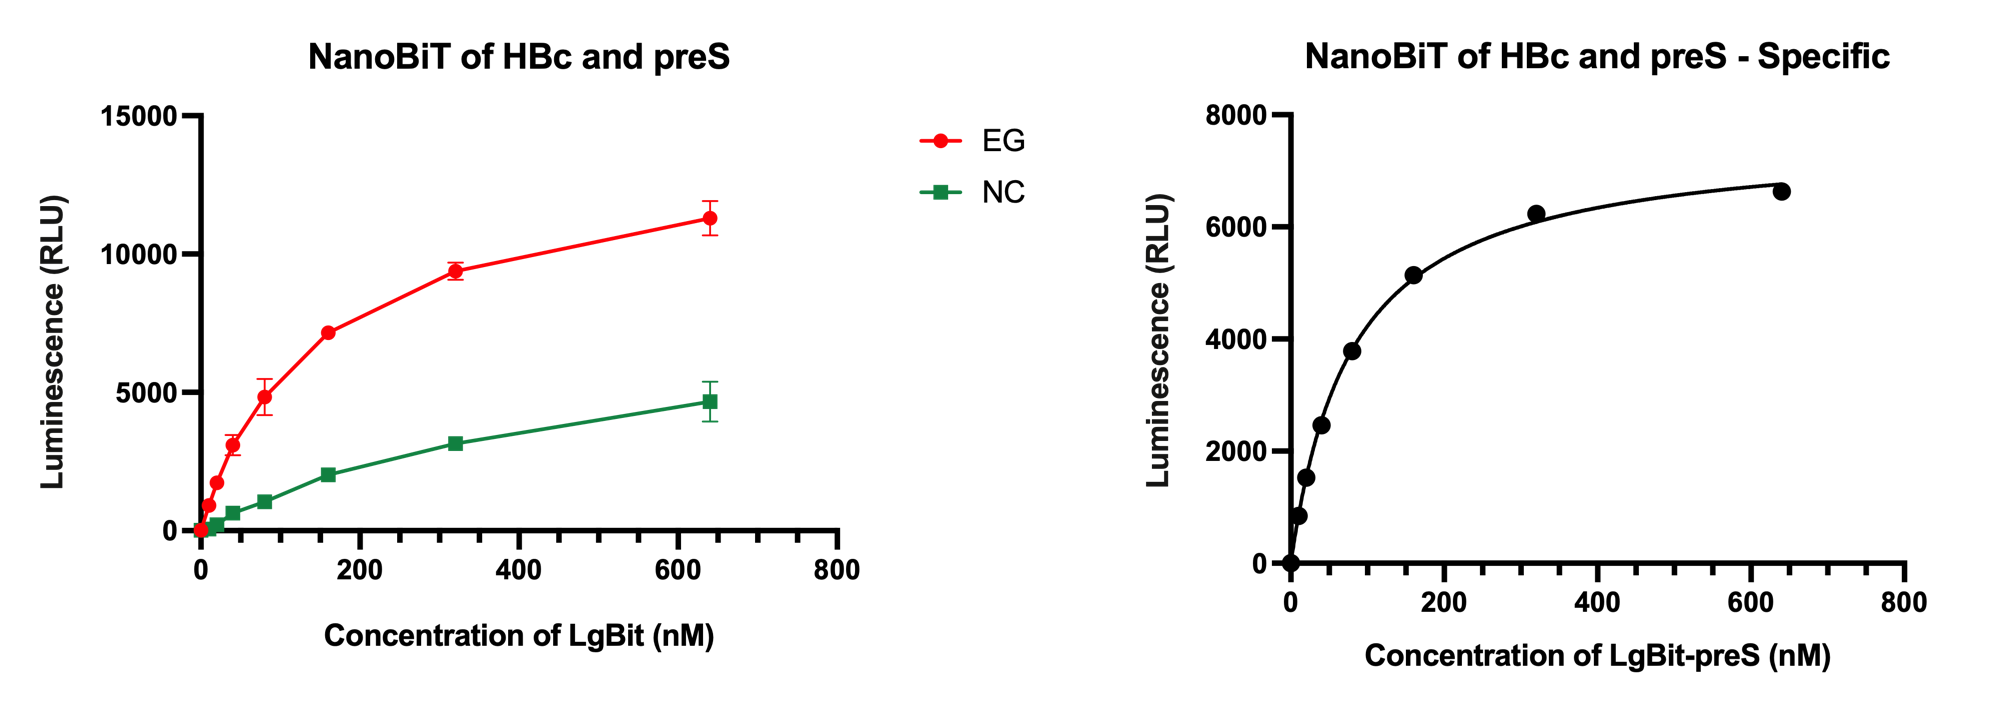
\includegraphics[width=0.52\textwidth]{figures/result/result_41.png}
  \hfill
  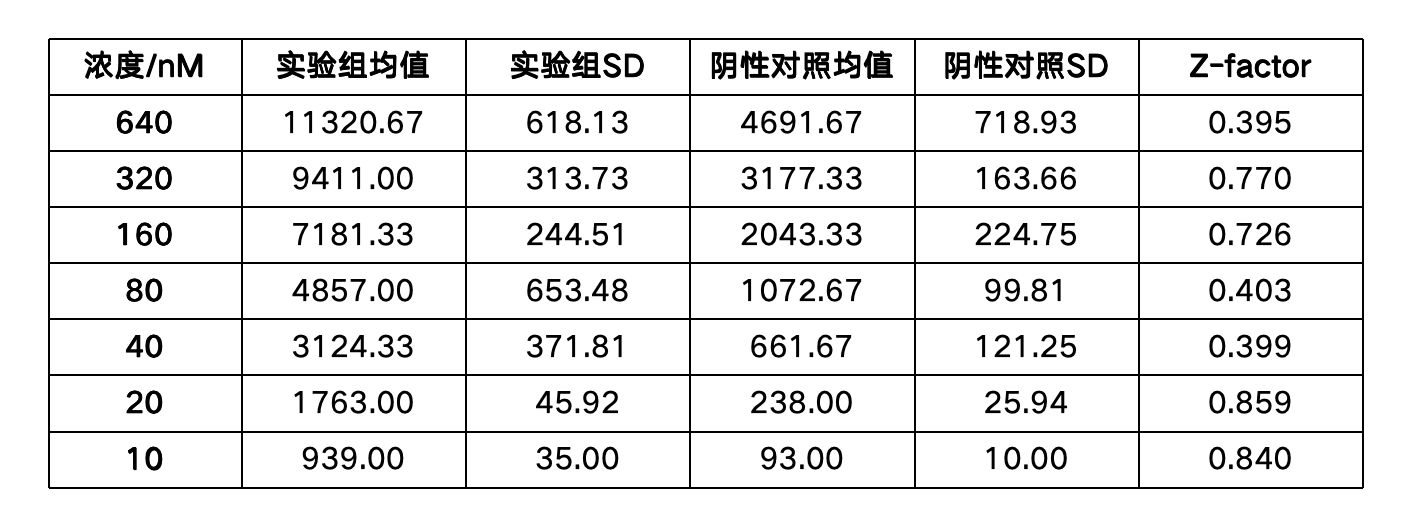
\includegraphics[width=0.38\textwidth]{figures/result/result_42.png}
  \caption{使用新纯化HBVCp182-SmBiT重复NanoBiT滴定实验。实验组信号随LgBiT-preS浓度升高而增加，扣除阴性对照后的特异性信号呈饱和趋势。}
  \label{fig:repurified-hbvcp182-nanobit-titration}
\end{figure}

\subsection{含foldon构建体条件下的小分子抑制实验}

在上述滴定结果基础上，首先使用含foldon的LgBiT-preS体系检测候选小分子对HBc--preS相互作用的影响。初筛中比较了Triton X-100、NP-40和香叶醇对NanoBiT发光信号的影响。直接加入小分子时，三种小分子均未产生充分清晰的抑制窗口。Triton X-100和NP-40的实验组信号在高浓度区间有一定下降，但阴性对照也发生轻度变化；香叶醇处理下的特异性信号波动更明显，整体趋势不够稳定。

这一结果提示，在直接加药条件下，小分子对HBc--preS相互作用的抑制不易被稳定观察。可能原因包括候选小分子与HBVCp182-SmBiT接触时间不足、检测浓度范围尚未覆盖有效区间，以及含foldon的LgBiT-preS构建体可能以多价形式增强表观结合，从而降低小分子竞争效应的可观察性。

\begin{figure}[htbp]
  \centering
  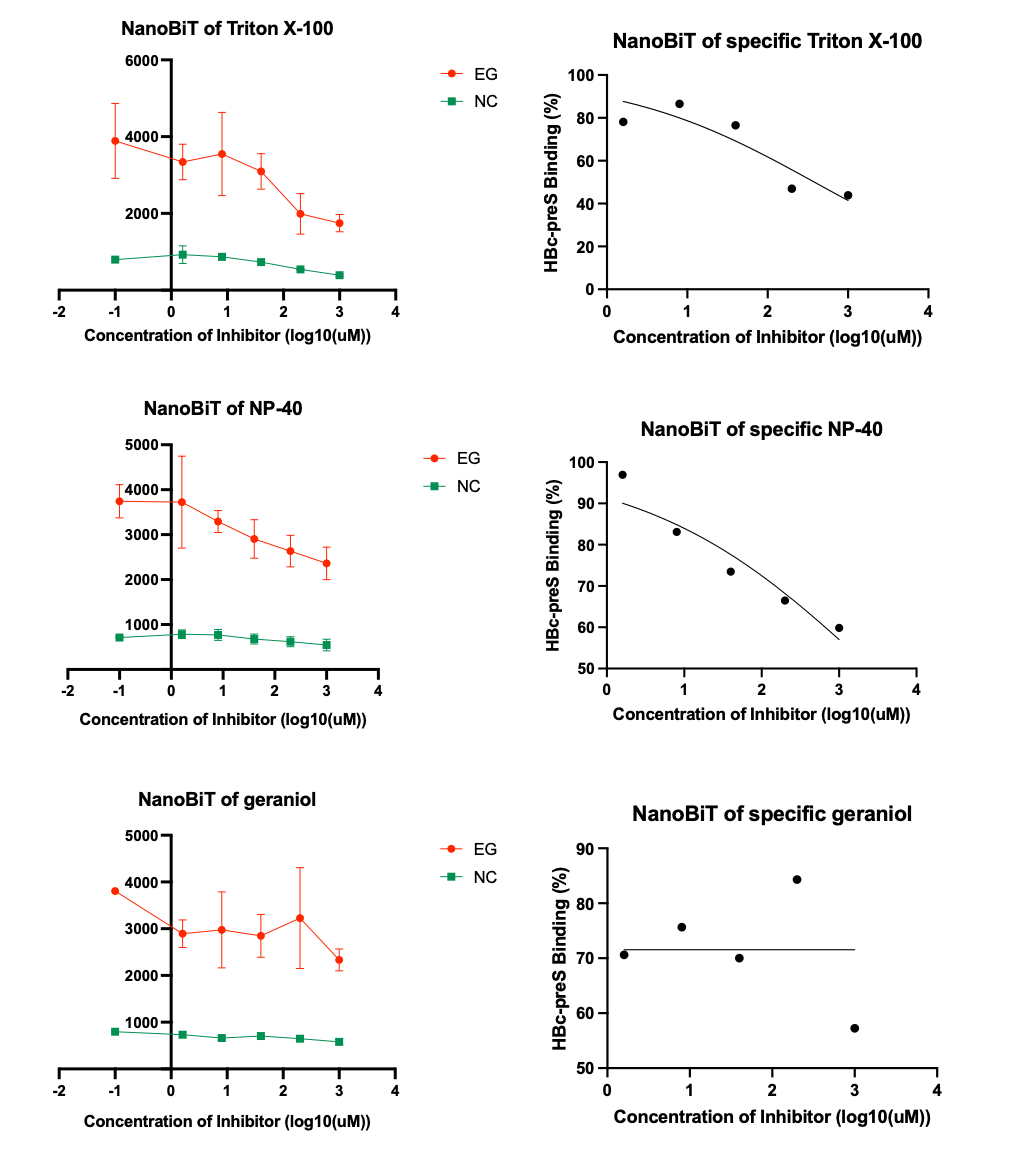
\includegraphics[width=0.70\textwidth]{figures/result/result_43.png}
  \caption{含foldon构建体条件下的小分子抑制初筛。直接加入Triton X-100、NP-40和香叶醇时，HBc--preS特异性信号未形成稳定清晰的剂量依赖性抑制窗口。}
  \label{fig:foldon-inhibitor-initial}
\end{figure}

为增强小分子与HBVCp182-SmBiT的接触，后续实验改为先将候选小分子与HBVCp182-SmBiT预先孵育，再加入LgBiT-preS或LgBiT阴性对照进行检测，并提高抑制剂浓度范围。在该条件下，Triton X-100、NP-40和香叶醇对HBc--preS发光信号的抑制趋势更加明显，尤其在高浓度区间，实验组信号出现更大幅度下降，扣除阴性对照后的相对结合百分比也呈下降趋势。

尽管如此，含foldon体系仍不适合直接计算准确的表观亲和力或IC$_{50}$。当前使用的GST-LgBiT-preS 87--114-foldon构建体含有foldon结构域，可能诱导三聚化并增强多价结合；同时GST标签本身也具有二聚化倾向。这些因素可能提高体系的表观亲和力和发光信号，使小分子抑制被部分掩盖，也使剂量--反应曲线不能直接反映单价HBc--preS相互作用。因此，后续实验进一步转向不含foldon的LgBiT构建体，并尝试降低GST标签二聚化带来的影响。

\begin{figure}[htbp]
  \centering
  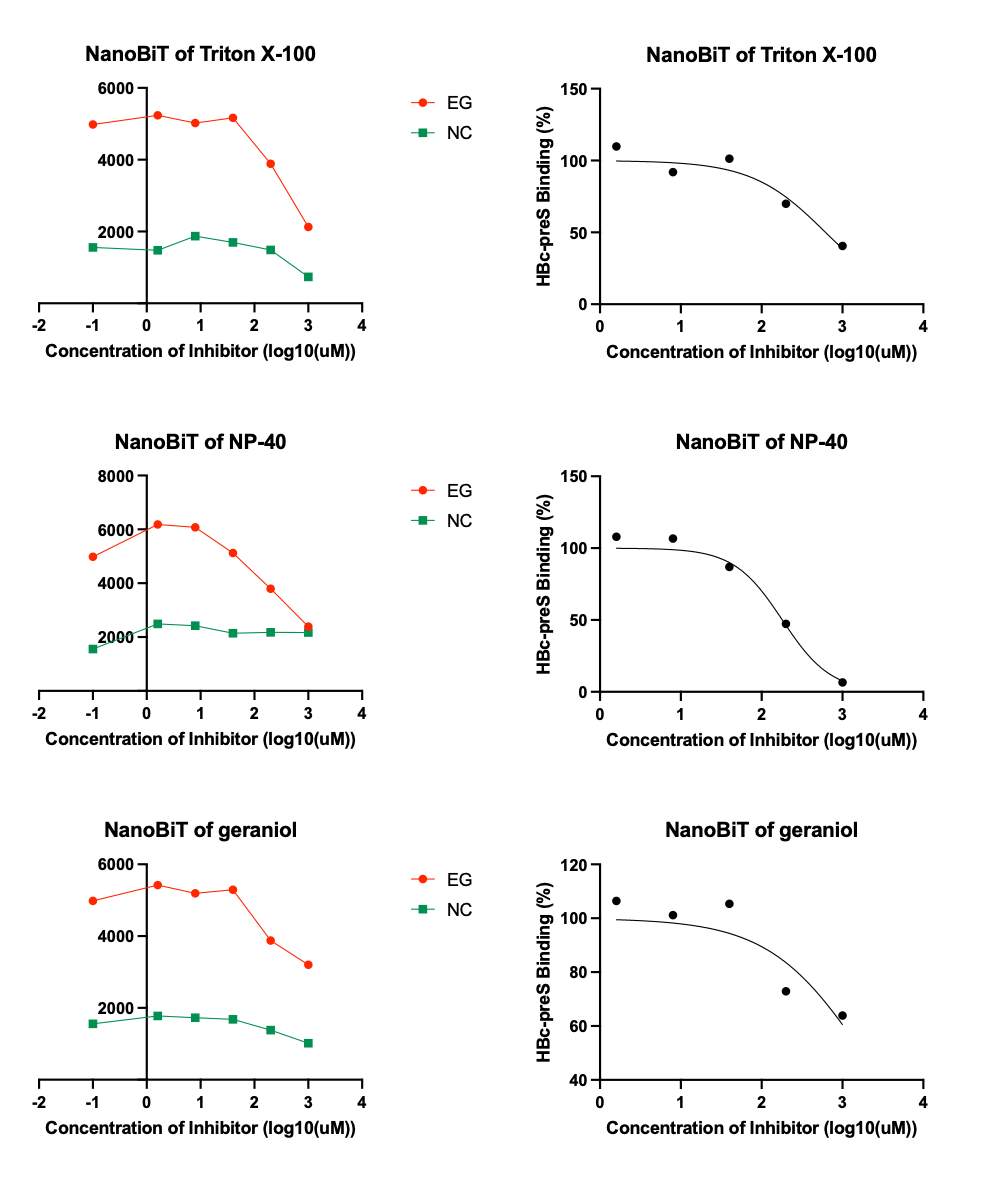
\includegraphics[width=0.70\textwidth]{figures/result/result_44.png}
  \caption{预孵育并提高小分子浓度后的含foldon体系抑制实验。高浓度区间实验组信号和相对结合百分比下降更明显，但foldon和GST相关多价效应限制了定量解释。}
  \label{fig:foldon-inhibitor-preincubation}
\end{figure}

\subsection{不含foldon的LgBiT构建体制备与NanoBiT滴定}

为降低foldon介导的多聚化效应，进一步制备了不含foldon的GST-LgBiT-preS 87--114-His和GST-LgBiT-His构建体。GST亲和纯化结果显示，GST-LgBiT-preS 87--114-His可在GST柱洗脱组分中观察到较清晰的目标条带，说明该构建体能够被GST柱有效捕获并洗脱。相比之下，GST-LgBiT-His在GST柱洗脱组分中回收较少，而流穿液中仍可见目标大小附近条带，提示该蛋白在当前条件下不易通过GST柱充分回收。

为提高阴性对照蛋白产量，进一步从GST柱流穿液出发，通过His标签富集和Q HP柱纯化获得GST-LgBiT-His。Q柱图谱中约16.03 mL处出现明显主峰，SDS-PAGE显示16--22管附近存在较集中的GST-LgBiT-His条带，说明补充纯化策略可获得足够的阴性对照蛋白用于后续实验。

\begin{figure}[htbp]
  \centering
  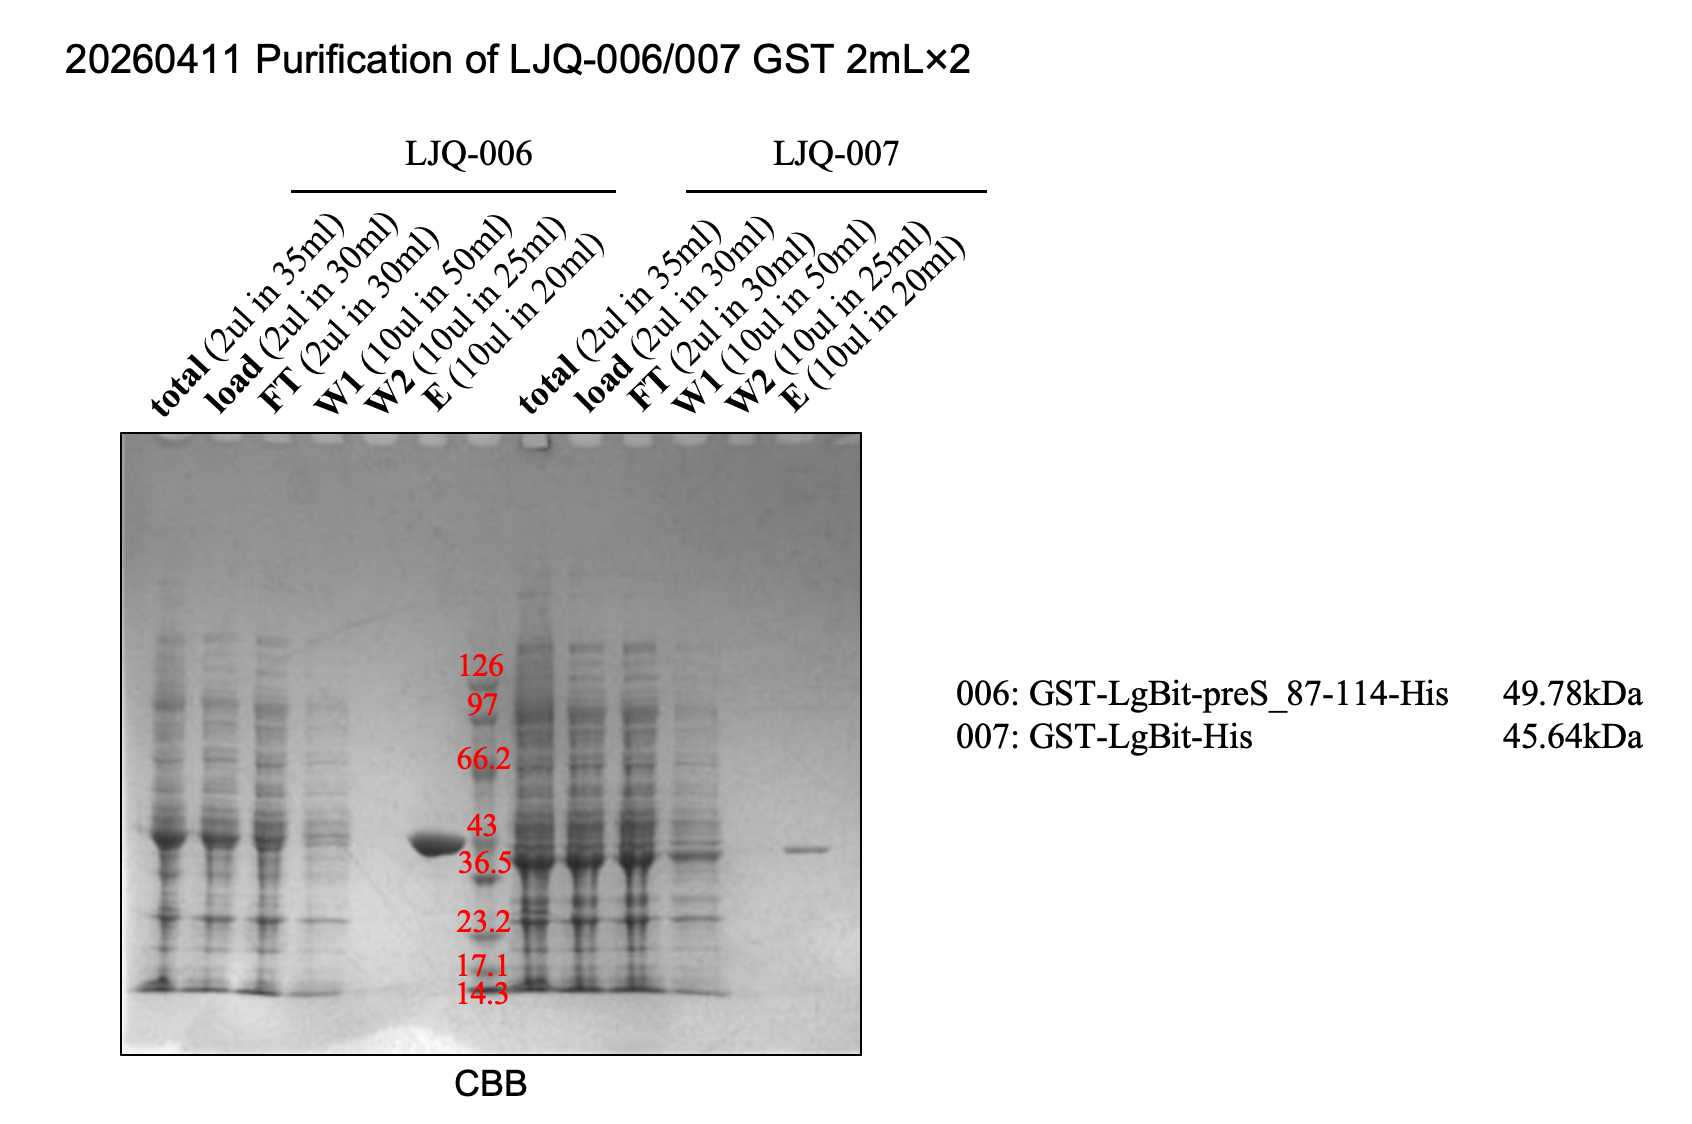
\includegraphics[width=0.58\textwidth]{figures/result/result_45.png}
  \caption{不含foldon的GST-LgBiT-preS 87--114-His和GST-LgBiT-His的GST柱纯化结果。GST-LgBiT-preS 87--114-His在洗脱组分中较为明显，而GST-LgBiT-His回收效率较低。}
  \label{fig:foldon-free-gst-purification}
\end{figure}

\begin{figure}[htbp]
  \centering
  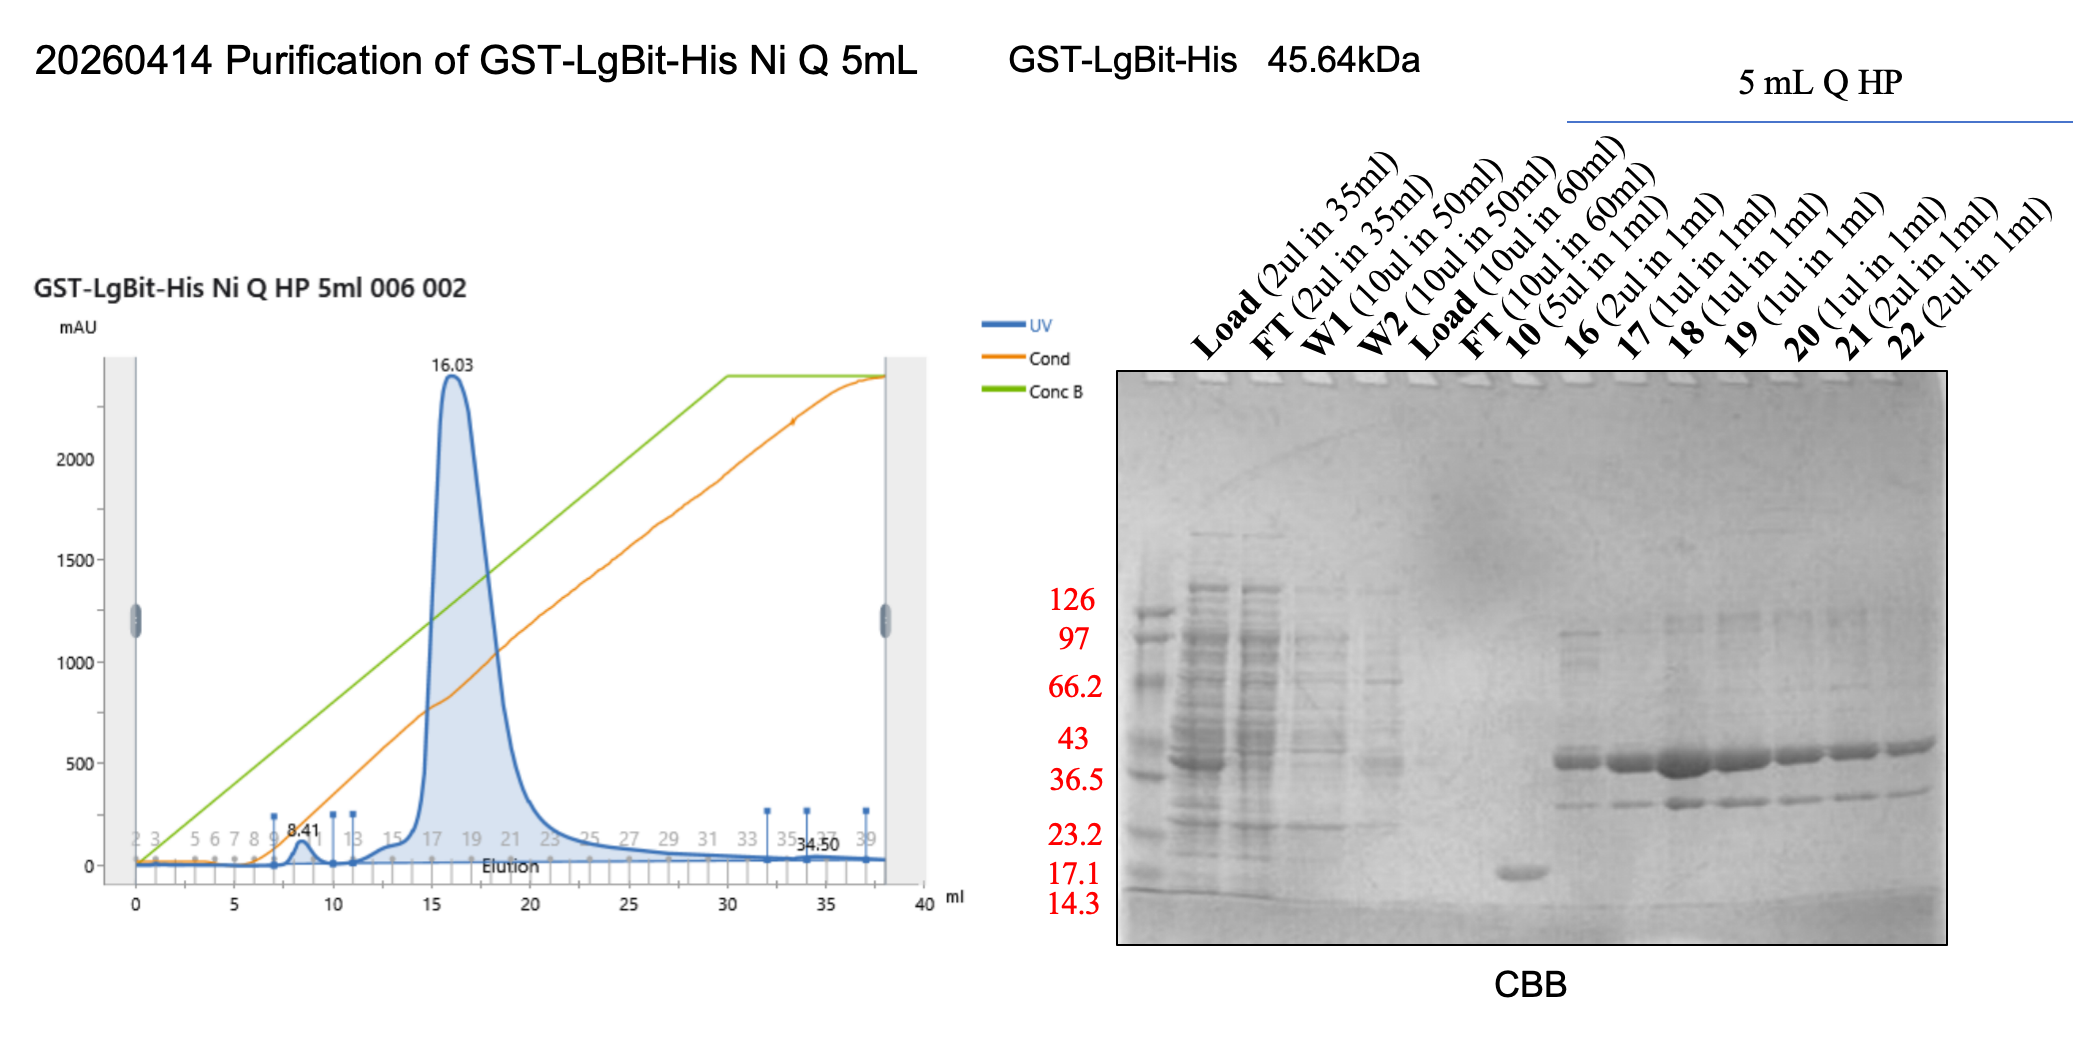
\includegraphics[width=0.82\textwidth]{figures/result/result_46.png}
  \caption{GST-LgBiT-His从GST柱流穿液出发的进一步纯化。Ni柱富集和Q HP柱纯化后，可获得用于后续NanoBiT检测的阴性对照蛋白。}
  \label{fig:gst-lgbit-his-further-purification}
\end{figure}

使用新纯化的不含foldon构建体重复HBc--preS NanoBiT滴定实验。与含foldon体系相比，不含foldon的LgBiT-preS不再具有三聚化带来的多价优势，因此需要更高浓度才能产生足够的特异性发光信号。实验组信号随着LgBiT-preS浓度增加而持续上升，阴性对照维持在较低水平但仍具有一定浓度依赖背景。扣除阴性对照后，特异性信号逐渐升高并呈现弯曲趋势，说明该体系仍可检测HBc--preS相互作用，但表观结合强度低于含foldon体系。

根据不同浓度范围的滴定结果，后续小分子抑制实验选择1000 nM LgBiT作为工作浓度。该浓度能够提供清楚的实验组与阴性对照分离，同时保留可观察的抑制空间；若浓度过低，信号窗口不足，而浓度过高则可能增加背景并削弱抑制剂引起的相对变化。

\begin{figure}[htbp]
  \centering
  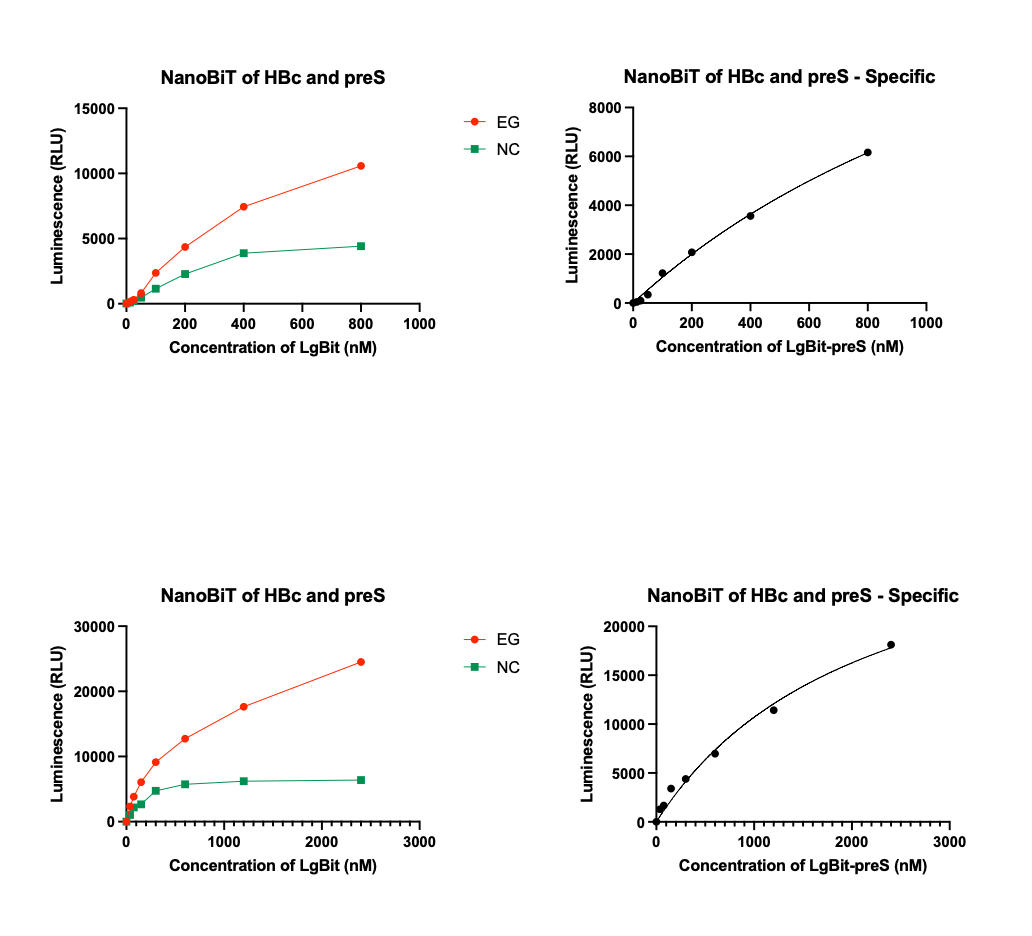
\includegraphics[width=0.76\textwidth]{figures/result/result_47.png}
  \caption{不含foldon体系下的HBc--preS NanoBiT滴定结果。实验组信号随LgBiT-preS浓度升高而增加，提示该体系可用于后续小分子抑制检测。}
  \label{fig:foldon-free-nanobit-titration}
\end{figure}

\subsection{不含foldon体系下的小分子抑制结果与GST标签影响}

在不含foldon体系中重新检测Triton X-100、NP-40和香叶醇对HBc--preS结合的影响。结果显示，三种小分子在高浓度区间均使实验组发光信号下降，其中Triton X-100和香叶醇的高浓度抑制趋势较为明显，NP-40的抑制曲线相对平缓且波动较大。扣除阴性对照后，Triton X-100和香叶醇的特异性结合百分比下降更清楚，说明不含foldon体系较含foldon体系更容易显示小分子作用。

需要注意的是，高浓度小分子存在时，阴性对照信号也发生改变，提示这些分子可能不仅影响HBc--preS结合，也可能影响蛋白稳定性、NanoLuc片段互补效率或检测体系背景。因此，在目前数据基础上不宜直接给出IC$_{50}$。后续若进行定量拟合，需要加入NanoBiT片段互补本身的控制、蛋白聚集或变性控制，以及多次独立重复，并在背景受控的浓度区间内进行分析。

\begin{figure}[htbp]
  \centering
  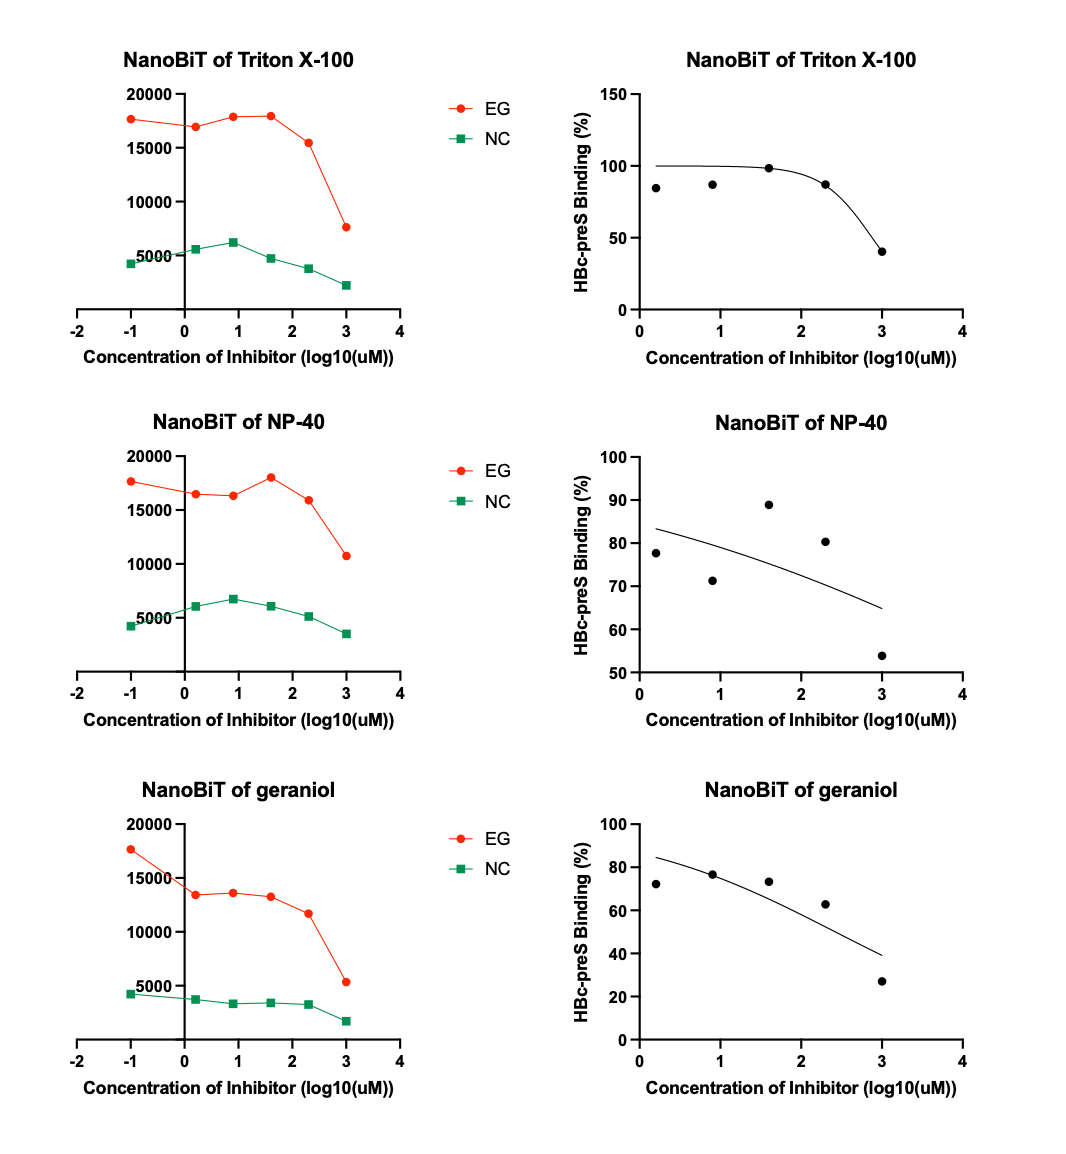
\includegraphics[width=0.74\textwidth]{figures/result/result_48.png}
  \caption{不含foldon体系下的小分子抑制实验。Triton X-100和香叶醇在高浓度区间显示更明显的相对抑制趋势，但阴性对照背景变化提示仍需进一步控制体系背景。}
  \label{fig:foldon-free-inhibitor-assay}
\end{figure}

由于GST标签本身可形成二聚体，可能使LgBiT-preS或LgBiT阴性对照发生非目标性聚集，从而影响NanoBiT信号解释，因此进一步使用PPase去除GST标签。SDS-PAGE结果显示，酶切后样品中出现与GST、LgBiT-preS和LgBiT相对应的条带；与未酶切样品相比，目标融合蛋白发生明显迁移变化，说明GST标签去除基本成功。该步骤为后续更接近单体状态的preS突变体比较提供了必要条件。

\begin{figure}[htbp]
  \centering
  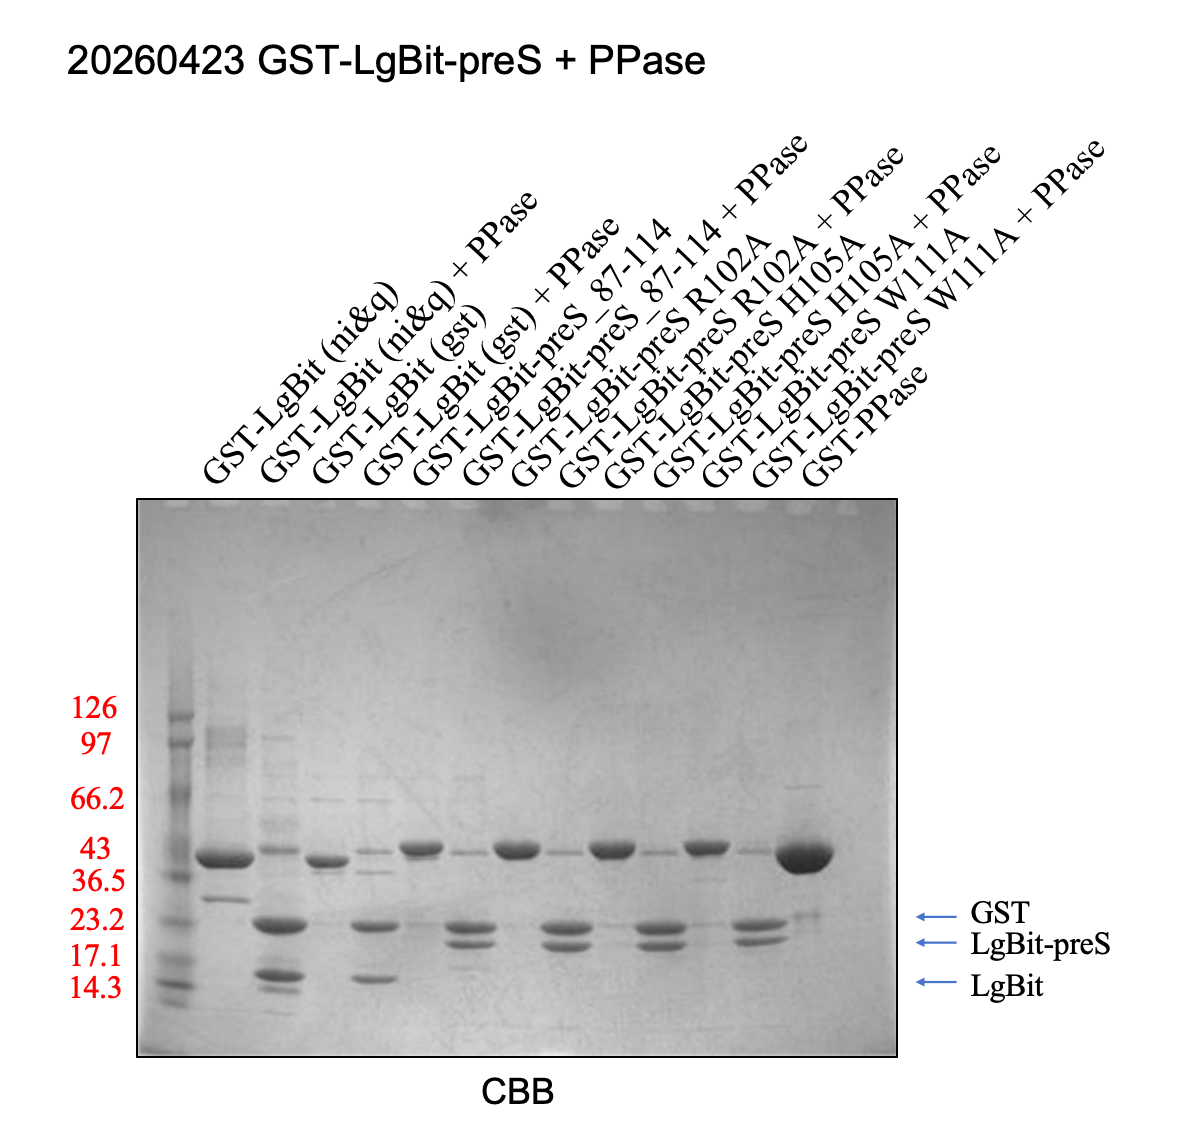
\includegraphics[width=0.58\textwidth]{figures/result/result_49.png}
  \caption{PPase切除GST标签的SDS-PAGE分析。酶切后可观察到GST、LgBiT-preS和LgBiT相关条带，提示GST标签去除基本成功。}
  \label{fig:ppase-gst-cleavage}
\end{figure}

\subsection{去除GST标签后preS突变体与HBc结合能力比较}

最后，利用酶切后的LgBiT-preS蛋白比较wild-type preS 87--114及R102A、H105A和W111A突变体与HBVCp182-SmBiT的结合能力。结果显示，wild-type preS 87--114在整个LgBiT浓度范围内均产生最高发光信号，且随浓度升高持续增加。相比之下，三个突变体的信号均显著降低，并接近或仅略高于LgBiT阴性对照。

从趋势上看，R102A和H105A的结合信号下降最明显，整体接近阴性对照水平；W111A仍保留一定残余信号，但明显低于wild-type preS 87--114。该结果表明R102、H105和W111均参与preS 87--114与HBc的结合界面，其中R102和H105对结合贡献尤其明显。更重要的是，该实验说明经过foldon去除和GST酶切后的NanoBiT体系能够区分不同preS突变体的结合能力，具有用于机制分析和后续突变筛选的可行性。

\begin{figure}[htbp]
  \centering
  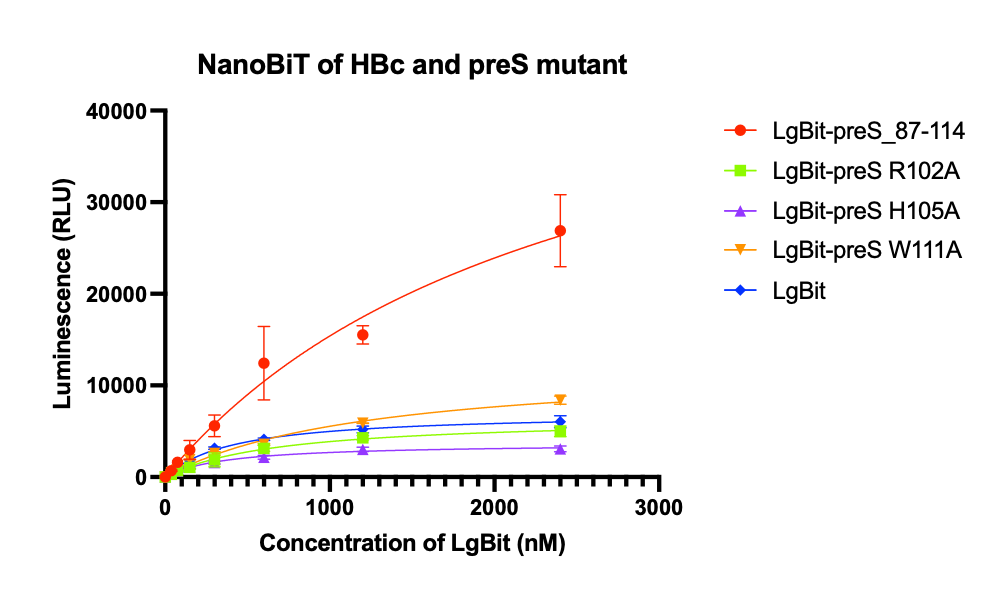
\includegraphics[width=0.56\textwidth]{figures/result/result_50.png}
  \hfill
  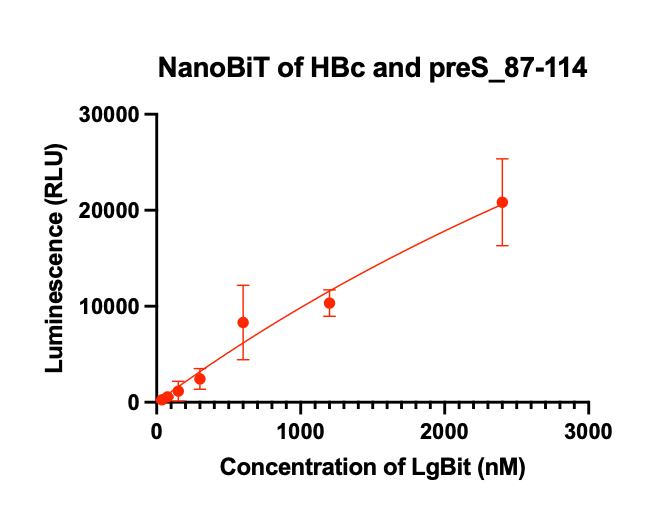
\includegraphics[width=0.36\textwidth]{figures/result/result_51.png}
  \caption{去除GST标签后wild-type preS 87--114与preS突变体的NanoBiT比较。R102A、H105A和W111A均显著降低HBc--preS互作信号，其中R102A和H105A下降最明显。}
  \label{fig:pres-mutant-nanobit}
\end{figure}

\section{本章结果小结}

\subsection{ELISA体系的主要结论}

本章首先建立并比较了HBc--preS体外互作检测体系。三种ELISA构型分别从HBc直接包被、StrepXT捕获preS和抗core Fab捕获HBc三个角度优化检测流程，但均受到非特异背景高、信号窗口窄或重复性不足的限制，难以作为后续突变体比较和小分子抑制评价的主要平台。相比之下，NanoBiT体系能够在较少洗涤干扰的条件下检测HBVCp182与preS 87--114之间的相互作用，并在合适浓度下获得较好的实验组--阴性对照分离。

\subsection{NanoBiT平台的优化结论}

后续实验进一步优化了NanoBiT平台。重新纯化HBVCp182-SmBiT提高了体系稳定性；含foldon体系可检测HBc--preS相互作用并初步观察小分子抑制趋势，但foldon和GST带来的多价效应限制了定量解释；不含foldon并进一步去除GST标签的体系更适合分析单价preS片段与HBc的相互作用。

\subsection{preS关键残基验证与平台意义}

基于该优化体系，preS R102A、H105A和W111A突变均显著降低HBc--preS互作信号，支持这些残基在结构界面中的关键作用。整体来看，本研究已建立可用于机制验证和候选小分子初步评价的非感染性体外NanoBiT平台，为后续围绕HBc--preS界面的抗病毒策略研究提供了实验基础。
